\documentclass[
   catalan,
%   handout,
   ]{beamer}
\usepackage{babel}
\usepackage[utf8]{inputenc}
\usepackage[style=authoryear,sortcites=true]{biblatex}
\newcommand{\bibendash}{--}
\usepackage{cclicenses}
\usepackage{appendixnumberbeamer}
\usepackage{tikz}
\usetikzlibrary{shapes,arrows,positioning}
\usepackage{pgfplots}
%\usetikzlibrary{dateplot}  
%\usetikzlibrary{pgfplots.groupplots}






% \pgfplotsset{
%    rrbtimeseries/.style={
%         % date coordinates in=x,
%         ylabel=Temperature (K),
%         % legend style={font=\footnotesize},
%         % tick label style={font=\footnotesize},
%         % every axis x label/.style={
%         %   at={(1.3,0)},
%         %   anchor=north,
%         %   },
%         % label style={font=\footnotesize},
%         % xticklabel style= {rotate=17,anchor=north east},
% %        every axis title shift=0pt,
% %        max space between ticks=15,
%        %  every mark/.append style={mark size=6},
%        %  major tick length=0.1cm,
%        %  minor tick length=0.066cm,
%        %  very thin,
%        %  every axis legend/.append style={
%        %    at={(1.2,0)},
%        %    anchor=south east,
%        %    draw = none},
%        % legend columns = 4,
%        % unbounded coords=jump, %v>1.4
%     },

%   % rrbrs/.style={
%   %       rrbtimeseries,
%   %       width = \textwidth,
%   %       height = 0.25\textwidth,
%   %       every axis x label/.style={
%   %         at={(1.3,-1)},
%   %         anchor=north,
%   %         },
%   %       ylabel = {},  
%   %       max space between ticks=50,
%   %       every axis legend/.append style={
%   %         at={(1,-1.1)},
%   %         anchor=north east,
%   %         draw = none},
%   %       title style={font=\small,below,anchor=north,fill=white},
%   %   },
%  }




\pgfplotsset{
   timeseries/.style={
        date coordinates in=x,
        ylabel=Temperature (K),
        legend style={font=\footnotesize},
        tick label style={font=\footnotesize},
        every axis x label/.style={
          at={(1.3,0)},
          anchor=north,
          },
        label style={font=\footnotesize},
        xticklabel style= {rotate=17,anchor=north east},
%        every axis title shift=0pt,
%        max space between ticks=15,
        every mark/.append style={mark size=6},
        major tick length=0.1cm,
        minor tick length=0.066cm,
        very thin,
        every axis legend/.append style={
          at={(1.2,0)},
          anchor=south east,
          draw = none},
       legend columns = 4,
    },
    rd/.style={
        timeseries,
        every axis x label/.style={
          at={(1.3,-1)},
          anchor=north,
          },
        label style={font=\footnotesize},
        ylabel = {},
        width=17cm,
        height=3.5cm,   
        max space between ticks=50,
        every axis legend/.append style={
          at={(1,-1.1)},
          anchor=north east,
          draw = none},
        title style={font=\small,below, at={(0.7,1.7)},anchor=north,fill=white},
    }
}


%        unbounded coords=jump, %v>1.4
%        unbounded coords=discard, %v>1.4


%http://tex.stackexchange.com/questions/46422/axis-break-in-pgfplots

%http://tex.stackexchange.com/questions/52409/insert-a-separate-mark-inside-a-pgfplots-graph
\usetikzlibrary{dateplot}

\mode<beamer>
{
  \usetheme{Madrid}
  \useoutertheme[subsection=false]{smoothbars}
  \setbeamercovered{transparent}
  \beamertemplatenavigationsymbolsempty
}

\mode<handout>
{
  \usepackage{pgfpages}
  \pgfpagesuselayout{8 on 1}[a4paper,border shrink=5mm]
  \setbeamercolor{background canvas}{bg=black!5}
  \usetheme{Madrid}
  \useinnertheme{default}
  \usecolortheme{dove}
}


% \makeatletter
% \patchcmd{\slideentry}
% {}%{\advance\beamer@tempdim by -.05cm}
% {}%{\advance\beamer@tempdim by\beamer@vboxoffset\advance\beamer@tempdim by\beamer@boxsize\advance\beamer@tempdim by 1.2\pgflinewidth}
% {}
% {}
% \patchcmd{\slideentry}
% {}%{\kern\beamer@tempdim}
% {}%{\advance\beamer@tempdim by 2pt\advance\beamer@tempdim by\wd\beamer@sectionbox\kern\beamer@tempdim}
% {}
% {}
% \makeatother


\bibliography{../bibliografia}
\renewcommand*{\bibfont}{\footnotesize}
\bibparsep 0.2cm
\bibhang 0.25cm
%\ExecuteBibliographyOptions{
%  isbn=false,url=false,doi=false,firstinits=true,abbreviate=true
%}


%------------- capçaleres pdf -----------

\title%
   [Model multiresolució per a sèries temporals]%
   {Disseny i modelització d'un sistema de gestió multiresolució per a sèries temporals}

\author[A. Llusà]
{%
  Aleix Llusà Serra \\
  {\footnotesize Direcció: Teresa Escobet Canal i Sebastià Vila-Marta}
}

\institute[Programa doct.\ ARV UPC]
{
  {\large Universitat Politècnica de Catalunya} \\
  Programa de Doctorat en Automàtica, Robòtica i Visió 
}


\date[Desembre 2015]
{Tesi Doctoral \\ Desembre 2015}


\subject{Defensa de tesi doctoral 2015}
\keywords{sèries temporals; model de dades; sistemes de bases de dades; sistemes de monitoratge}



\begin{document}

\begin{frame}[plain]
 \titlepage

 \begin{center}
   {\footnotesize \cc\bysa}
   {\tiny Aquest document està sotmès a una llicència de Reconeixement-CompartirIgual 3.0 de Creative Commons\\
     El codi font \LaTeX\ del document es troba a
     \url{http://escriny.epsem.upc.edu/projects/rrb/} }
  \end{center}

\end{frame}

\section*{Índex}
\begin{frame}{Índex}
 \tableofcontents
\end{frame}


\section{Introducció}



\section{Introduction}



Information collection processes are growing in quantity as a
consequence of the emergence of embedded systems and sensor networks.
Nowadays it is possible to collect large amounts of data to monitor
and control complex systems.  This information must be analysed and
prepared by information systems in order to detect eventual sensor
failures or malfunctions and, if it is possible, to reconstruct the
incorrect signals. Acquired data instance are bound to a timestamp,
therefore correctness criteria must include both data value and its
timestamp. The sequences of data values collected at specific
timestamps are formalised as time series.


Time series are defined as a collection of observations made
chronologically.  In general, time series come from a continuous
nature in which they are recorded at regular intervals, such as hourly
or daily, or at irregular intervals, such as recording when a pump is
open or closed.  One problem when dealing with time series data
results from the fact that these data are often voluminous
\cite{fu11,keogh08:isax}, as a result, efficiently storing and
accessing them can be complex. Moreover, this is specially critical
when developing small embedded systems, whose resources (capacity,
energy, processing and communications) suffer restrictions
\cite{yaogehrke02}.  Another problem is that the procedure of
processing and synthesising information becomes difficult if data is
not equi-time spaced.



Time series can be stored and managed by Structured Query Language
(\acro{SQL}) relational database management systems. However, some
authors \cite{dreyer94,schmidt95,stonebraker09:scidb,zhang11} notice
that the use of \acro{SQL} systems as a time series backend suffers
some drawbacks.  On the one hand, \emph{NoSQL} or \emph{NewSQL}
products are being developed in order to increase the performance and
flexibility of \acro{SQL} systems
\cite{atzeni13:relational_model_dead,stonebraker10,stonebraker09:scidb,zhang11},
however the continue acquisition nature of time series is an issue for
storing and analysing offline all the data \cite{keogh97}.

On the other hand, compression techniques for time series are
considered in the form of approximation to the original signal in
order to compute analysis such as similarity or pattern search
\cite{fu11,keogh01,last01} or in the form of compression and
aggregation approaches for massive data streams
\cite{cormode08:pods,bonnet01}. However, treating time series as data
streams does not consider adequately the time dimension nor computes
the evolution of aggregated parameters along time, which is
interesting for monitoring purposes.  On a similar approach,
\emph{RRDtool} \cite{rrdtool} is a system that stores time series
aggregated in different resolutions in order to compact data and to do
faster visualisations. However, \emph{RRDtool} is very specific and
has limited aggregation operations to applications of network
counters.



\subsection{Contribution}


%TSMS

This paper focuses on Data Base Management Systems \linebreak[4]
(\acro{DBMS}) that store and treat data as time series, usually known
as Time Series Data Base Management Systems (\acro{TSMS}),
\cite{dreyer94,last01}.  We introduce a new data model named
multiresolution \acro{TSMS} (\acro{MTSMS}). This model organises data
in an aggregated way and  allows to store time series using
different time resolutions. It is designed to cope well with bounded
storage computers such as sensor systems.  

We describe the model in two separated submodels, one \acro{TSMS}
model mainly for describing time series basic concepts and operations
and the other a \acro{MTSMS} model for describing multiresolution over
time series. The model is described firmly rooted on set and
relational algebra as a formal theory for information systems.  It
also considers the time irregularities sampling of time series,
moreover it operates coherently with the time dimension of time
series.


% Our multiresolution definition is
% based on concepts of RRDtool but aims to generic applications and has
% more generic operators.


Multiresolution is proposed as a lossy storage solution that selects
only the needed information. The concept is similar to multimedia
lossy compression methods, where information can be discarded in
favour of size, but applied to time series.  Multiresolution is an
aggregation of data that stores the evolution of the parameters along
time, which is more related to the needs of monitoring. However, as a
lossy storage solution, the multiresolution schema has to be decided
for each application, deciding what approximate queries will be needed
to resolve. We formalise aggregation functions as an independent
object of the main model. Therefore, users can define new operations
and other aggregation methods from other fields such as data
streaming or time series data mining.


A representation function concept of time series is also formalised, then
users can define different operators considering the behaviour of time
series in different contexts. Especially, it is important when defining
new aggregation operations that must consider different meanings of
the time series, i.e. \emph{RRDtool} specific counter time series
aggregations. Furthermore, we formalise representation as an
independent object of the main model.




\subsection{Outline}

This manuscript is organised as follows.  In
Section~\ref{sec:related-work} some related work concerning
\acro{TSMS} and \acro{MTSMS} are presented.  The motivation for
multiresolution is shown in Section~\ref{sec:features}.  The
\acro{TSMS} model is presented in Section~\ref{sec:model:TSMS} and the
\acro{MTSMS} model is presented in Section~\ref{sec:MTSMS}.  In
Section~\ref{sec:implementation} there is a implementation
for the \acro{TSMS}+\acro{MTSMS} model.  Section~\ref{sec:example} is
devoted to a real data multiresolution database example.  Finally,
Section~\ref{sec:concl-future-work} offers some conclusions.
\ref{sec:notation} shows main notation symbols.





\section{State of the art}
\label{sec:related-work}

In this section, related work to mutiresolution time series is
described in three parts: some database management systems
approaches for time series, compression techniques applied to time
series, and computations based on data streams.




\subsection{Database approaches}

Some authors treat \acro{TSMS} as a particular \acro{DBMS} field
\cite{last01}.  Segev and Shoshani \cite{segev87:sigmod} propose an
structured language for querying \acro{TSMS}. Their time series
structures include the notion of regularity and temporal
representation and their operations are \acro{SQL}-like.  Dreyer et
al.\ \cite{dreyer94} propose the requirements of special purpose
\acro{TSMS} and base the model on five basic structural elements:
events, time series, groups, metadata and time series bases. They
implement a \acro{TSMS} called \emph{Calanda} which includes calendar
operations, allows grouping time series and operating with simple
queries. They exemplify it with financial data. In \cite{schmidt95}
\emph{Calanda} is compared with temporal systems designed for time
series.



 
Others implement \acro{TSMS} with array database approaches.
\emph{SciDB} \cite{stonebraker09:scidb} and \emph{SciQL}
\cite{zhang11} are array database systems intended for science
applications, in which time series play a principal role. They
structure time series into arrays in order to achieve multidimensional
analysis and they store other data into tables.  \emph{SciDB} is based
on arrays which, according to the authors, allow to represent time
series.  In contrast, \emph{SciQL} defines time series as a mixture of
array, set, and sequence properties and exhibits some time series
managing characteristics that include time series regularities,
interpolation or correlation queries.
% However,
% difference between tables and arrays seems too physical and leads to
% ambiguity when representing time series.  
% Our TSMS model proposes time
% series as firmly based on relational algebra, clarifying this
% ambiguity and describing them coherently in terms of information
% systems theory.





Bitemporal \acro{DBMS}, sometimes referred directly as temporal data,
is a database field related with time. Bitemporal data manages
historical data and events in databases by associating pairs of
\emph{valid} and \emph{transaction} time intervals to data.
Bitemporal data and time series data are not exactly the same and so
can not be treated interchangeably \cite{schmidt95}, however, there
are some similarities that can be considered. Moreover, \acro{DBMS}
research represents bitemporal data as relations extended with time
intervals attributes and extends relational operations in order to
deal with related time aspects
\cite{jensen99:temporaldata,date02:_tempor_data_relat_model}.  We
formalise time series similarly as how bitemporal data is formalised
for relational \acro{DBMS}.
% On the other hand, some bitemporal time concepts might be taken
% into account by \acro{TSMS}, such as the discussions about time
% granularities.



\subsection{Compression techniques}


% As \acro{TSMS} suffer from problematic properties of time
% series, like the ones we describe in
% Section~\ref{sec:model:properties} mainly the huge data volume,
% compression techniques are used.  Next, we summarise some current work
% in \acro{TSMS} with compression.



\emph{RRDtool} from Oetiker, \cite{rrdtool,lisa98:oetiker}, is a free
software database management system. It is designed to be used for
monitoring systems. Because of this, it is focused to a particular
kind of data, gauges and counters, and it lacks general time series
operations. \emph{RRDtool} can store multiple time resolution data,
however Plonka et al.\ \cite{lisa07:plonka} evaluated \emph{RRDtool}
performance and found limitations when storing huge number of
different time series. They propose a caching system on top of
\emph{RRDtool} as a solution.  \emph{RRDtool} is extremely used by the
free software community so it inspired us to develop a model from its
main characteristics, that is now what we call multiresolution. A
similar approach is done by \cite{weigel10} in a system called
\emph{TSDS} that caches queries by aggregate parameters. They notice
that data needs to be shown over its full time range and not only
subsets of data as it is usually provided.  They develop the software
package \emph{TSDS} where time series are stored fully and then
requested by date ranges or by applying different filters and
operations to the time series data.  Our \acro{MTSMS} model is a generic
approach to the multiresolution features, we define it open so that
users can define any attribute aggregate functions.


Deri et al.\ \cite{deri12:tsdb_compressed_database} present
\emph{Tsdb}, a lossless compression storage \acro{TSMS} for time
series that share the same time instants of acquisition. Different
time series are stored grouped by the time of acquisition instead of
each time series isolated.  They compare \emph{Tsdb} with \emph{RRDtool} and
with a relational product. As a consequence of \emph{Tsdb} structure,
they achieve a better measure addition time but a worse global
retrieval time as data has to be contiguously regrouped. However, when
measures have same time this is seen as the same time series in a
\acro{MTSMS}, so it would be interesting to use this implementation
architecture of shared time arrays in \acro{MTSMS} for resolution subseries
with same delta time in order to achieve better performance requirements
when having much equal acquired time series.

% Therefore, as it is a very different approach from RRDtool we find it difficult to compare both in these performance requirements. 
% He only evaluates compression performance but we think that a global
% evaluation of compression plus descompression must be done. MTSMS
% are not aimed to be a replacement for offline long time storage
% systems that are rarely queried and then queries can be slow but
% have tot be exact. MTSMS are adequate to stream processing and
% resolving queries with less data than original and so they are
% quicker but give information previously selected.


There are other lossy compression techniques for time series devoted
to the optimal approximation representation, that is finding the
compromise between least data that can reconstruct the original signal
with least error. Keogh et al.\ \cite{keogh01} cite some possible
approximation representations for time series such as Fourier
transforms, wavelets, symbolic mappings or piecewise linear
representation. They remark this last one as very usual due to its
simplicity and develop a system called \emph{iSAX}
\cite{keogh08:isax,keogh10:isax} in order to analyse and index massive
collections of time series. They describe that the main problem is in
the indexing of time series and they propose methods for processing
efficiently. The first method proposed is based on a constant
piecewise approximation. The time series representation obtained with
\emph{iSAX} allows reducing the stored space and indexing faster with
the same quality as other more complex representation methods.  These
compression techniques are candidates for being used as attribute
aggregate functions in the \acro{MTSMS} model, as instance it would be
interesting to define aggregations in the frequency domain of time
series.


% A Multiresolution Symbolic Representation of
% Time Series; Megalooikonomou, Faloutsos; 2005 proposes multiresolution by decomposing a signal in frequency subsequences and intended mainly to similarity searching. The objective is to reconstruct the original time series. 
 


% \paragraph{T-Time}  \textcite{assfalg08:thesis} shows a TSMS that can do similarity search, which is calculated as distances between time series. Mainly, two time series are marked as similar if they distance is less than a threshold in each interval. From this method efficient algorithms are developed and implemented in a program called T-Time, which is described in \cite{assfalg08:ttime}.

 


\subsection{Data stream}



There are other \acro{TSMS} specifically designed for a particular
field requirements.  \emph{Cougar} \cite{bonnet01} is a sensor
database system that has two main structures: one for sensor
properties stored into relational tables and another for time series
stored into data sequences from sensors. Time series have specific
operations and can combine relations and sequences. \emph{Cougar}
target field is sensor networks, where data is stored distributed in
different locations. Queries are resolved combining sensor data in a
data stream abstraction that improves processing performance.

Time series as data streams are also considered when aggregating
statistically data in order to do fast approximate queries with
compressed data, Cormode et al.\ \cite{cormode08:pods} develop
aggregation techniques that consider giving more weight to recent
information.  Our \acro{MTSMS} model applies a similar approach of
weighting more recent data but specifically to time series, with
multiple aggregations and considering time irregularities.


% Our MTSMS model can also be thought as an stream processor if measures
% are added in time order, there is no possibility of update operations,
% buffer time series become of unity cardinality, and aggregate
% functions are limited to stream capabilities ones.  
% As instance,
% RRDtool can be considered stream oriented and its consolidation
% process is done at the same time of inserting new measures.





\section{Multiresolution motivation}
\label{sec:features}

A \acro{TSMS} is a special purpose \acro{DBMS} devoted to store and
manage time series.  The main objective of \acro{TSMS} is to gather
two areas of study: time series analysis and \acro{DBMS}.  Time series
analysis formalises a great amount of algorithms and methodologies
that apply to time series, with a main focus on improving
efficiency. \acro{DBMS} theory formalises systems that store and
operate with data, currently the relational model is the referent
\cite{date:introduction}.



In time series analysis there are some common generic operations.
Most of these operations deal with the time given the nature of data.
Usual operations include querying time intervals, finding time
correlations, or calculating distances between two time series. In
all these operations \acro{TSMS} must consider the temporal coherence
of the time series.  In the context of statistics, aggregation of time
series is also a common operation. Aggregate means to summarise a time
series subset by a smaller set of measures. Statistic indicators like
the mean, the maximum, or the mode, for instance, summarise time
series into one only measure.

In the discrete context, a time series is defined as a set of value
and time pairs. Furthermore, a time series has a continuous nature as
it comes from a phenomena evolution along time. As a result,
\acro{TSMS} operations may deal with this time series nature by
methods of interpolation or approximation.


A \acro{MTSMS} proposes a \acro{TSMS} with multiresolution
capabilities.  A \acro{MTSMS} schema represents a time series using a
set of different resolutions.  The multiresolution concept comes from
thoroughly analysis of \emph{RRDtool} \cite{rrdtool}. Our objectives
have been to formalise the main concepts into an abstract model and to
include more genericity in order to describe \acro{MTSMS} as fully
\acro{TSMS}.

%Then we will be able to apply these systems to other applications.

As a summary, \acro{MTSMS} improve \acro{TSMS} features in various aspects:
\begin{itemize}

\item Voluminous data. Monitoring systems capture a huge amount of
  data from sensors. In order to be able to process this information,
  data volume must be reduced. One of the features of the
  multiresolution approach is to select and store only the most
  interesting segments of data. This segments are seen as different
  resolutions for the same time series and the user can configure how
  they are extracted and summarised by defining different time steps
  and functions. Multiresolution can also be useful when graphing time
  series allowing the user to select the best time range and time
  step that fits into the screen; there is no need to process with
  more quantity of data than the one that can be
  shown.% In figure~\ref{fig:mtsms:sequence} there is an example of
  % extracting two resolutions: one every three units of time and
  % another every five.

\item Data validation. Monitoring systems capture data but can occur
  some drawbacks that will affect later the process of time series
  analysis. Main problems are found when monitors can not capture
  data, known as gaps, or capture data erroneously, such as outlayers
  \cite{quevedo10}.  The multiresolution attribute functions is
  designed to cope well with validating, filtering and reconstructing
  with this unknown data in order to keep a consistent
  historic.% In figure~\ref{fig:mtsms:sequence-irregular} an
  % example of a gap can be seen.

\item Data time regularising. Another monitoring side effect happens
  when the sampling rate is not constant, that is when the resulting
  data is not equi-time spaced. This no regularities can come from
  sampling jitters in periodic sampling or from no periodic
  event-based sampling \cite{kopetz11:realtime}. One multiresolution
  consolidation objective is to regularise the time interval when
  processing a time series, therefore each resulting time series
  segment has a regular time resolution. This regularising approach
  could also be used when the user wants to consult another resolution
  for a time series, such as changing periodic data from a month to a
  year step. % In
  % figure~\ref{fig:mtsms:sequence-irregular} an example of time
  % regularising can be seen.

\item Information summaries. Time series analysis typically focuses on
  reconstructing the original signal. However, the user objective in a
  database system is to consult some information. The multiresolution
  approach allows a lossy compression storage solution for data. Therefore
  it can be regarded as to extracting the interesting information and
  then storing it. The selected information must be determined a
  priori assuming the context where the future queries will be done.
  % In
  % figure~\ref{fig:mtsms:sequence} there is an example of summarising by
  % mean attribute.
\end{itemize}


However sometimes it may also be useful to complement \acro{MTSMS}
with other \acro{DBMS}. Not only to store the original values as a
long-term deposit consulted offline, but also to store related
information to time series such as units of values, sensor
localisation, classification tags, last measured value, etc.



\subsection{Motivation example}
%We give a motivation example of multiresolution applied to a time series.  

Figure~\ref{fig:mtsms:sequence} shows an example of a multiresolution
summary for a time series. It shows a snapshot in time, suppose
between time 9 and 10. At the top of the figure there is a plot of a
time series with time axis in general units of time (u.t.) and with
value axis in undetermined units. The 'now' point shows when the
snapshot has been taken, so the time before is the past and the time
after is the future, which is grey coloured. The \emph{init} point
shows when the database system has started sampling, so data in time
before is unknown; the starting point is indicated as zero u.t.\ and
the earlier unknown time points have negative units.


\begin{figure}
  \centering
  %\usetikzlibrary{positioning}
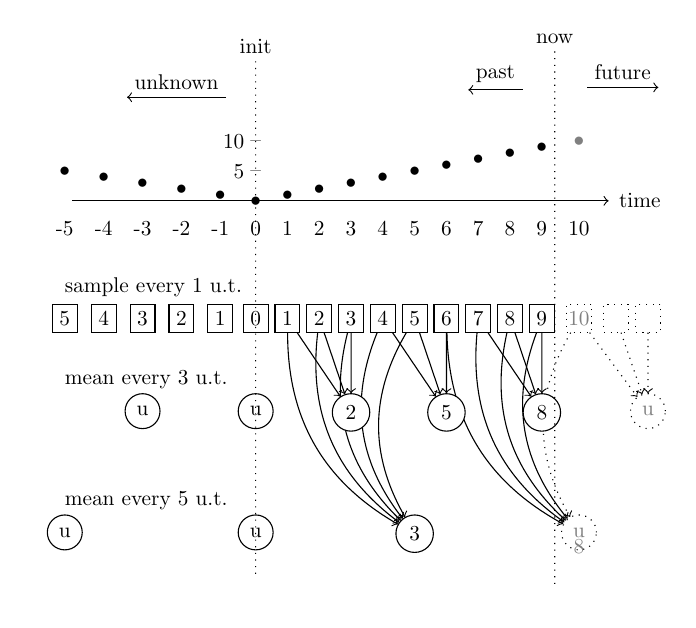
\begin{tikzpicture}[scale=0.77, every node/.style={transform shape}]

  %referencia
  \node (-6) {};

  \foreach \x in {-5,...,12}
  {
    \pgfkeys{/pgf/number format/.cd,int trunc}
    \pgfmathparse{abs(\x)}
    \let\absx=\pgfmathresult
    \pgfmathparse{\x-1}
    \let\antx=\pgfmathresult
    %time
    \node[node distance=1mm] (\x) [right=of \antx] 
    {\ifnum\x<11 \x \else \phantom{9} \fi};

    %graph values
    \node [above=\absx mm of \x] 
    {\ifnum\x=10 \color{gray} \fi \ifnum\x<11 $\bullet$ \fi};    

    %values
    % \node[rectangle,draw] (s\x) [below=of \x] 
    % {\ifnum\x<10 \pgfmathprintnumber{\absx} \else \phantom{9} \fi};
    \ifnum\x<10
    \node[rectangle,draw] (s\x) [below=of \x] 
    {\pgfmathprintnumber{\absx}};
    \else
    \node[rectangle,dotted,draw] (s\x) [below=of \x] 
    {\phantom{9}};
    \fi
  }

  \node [below=of 10] {\color{gray}10}; 
  

  
  %rd: 5s |inf| mean
  \node [circle,draw] (rd5-5) [below=3cm of s-5] {u};
  \node [circle,draw] (rd50) [below=3cm of s0] {u};
  \node [circle,draw] (rd55) [below=3cm of s5] {3};
  \node [circle,dotted,draw] (rd510) [below=3cm of s10] {\color{gray}u};
  \node [below=3.3cm of s10] {\color{gray}8};
 
  \draw[->,bend right] (s5) to (rd55);
  \draw[->,bend right] (s4) to (rd55);
  \draw[->,bend right] (s3) to (rd55);
  \draw[->,bend right] (s2) to (rd55);
  \draw[->,bend right] (s1) to (rd55);

  \draw[->,dotted,bend right] (s10) to (rd510);
  \draw[->,bend right] (s9) to (rd510);
  \draw[->,bend right] (s8) to (rd510);
  \draw[->,bend right] (s7) to (rd510);
  \draw[->,bend right] (s6) to (rd510);

  
  %rd: 3s |inf| mean
  \node [circle,draw] (rd3-3) [below=of s-3] {u};
  \node [circle,draw] (rd30) [below=of s0] {u};
  \node [circle,draw,fill=white] (rd33) [below=of s3] {2};
  \node [circle,draw,fill=white] (rd36) [below=of s6] {5};
  \node [circle,draw,fill=white] (rd39) [below=of s9] {8};
  \node [circle,dotted,draw] (rd312) [below=of s12] {\color{gray}u};

  \draw[->] (s3) to (rd33);
  \draw[->] (s2) to (rd33);
  \draw[->] (s1) to (rd33);

  \draw[->] (s6) to (rd36);
  \draw[->] (s5) to (rd36);
  \draw[->] (s4) to (rd36);

  \draw[->] (s9) to (rd39);
  \draw[->] (s8) to (rd39);
  \draw[->] (s7) to (rd39);

  \draw[->,dotted] (s12) to (rd312);
  \draw[->,dotted] (s11) to (rd312);
  \draw[->,dotted] (s10) to (rd312);



  %eixos
  \node (et0) [above=1mm of -5] {};
  \node (et12) [above=1mm of 11] {};
  \node [right=-2mm of et12] {time};
  \draw[->] (et0) to (et12);
  \node (y5) [above=5mm of 0] {--};
  \node [left=-1.5mm of y5] {5};
  \node (y10) [above=10mm of 0] {--};
  \node [left=-1.5mm of y10] {10};

  \node (inici) [above=4cm of s0] {init};
  \node (inici2) [below=4cm of s0] {};
  \draw[-,dotted] (inici) to (inici2);

  \node (fi) [above=4.4cm of s9.east] {now};
  \node (fi2) [below=4.4cm of s9.east] {};
  \draw[-,dotted] (fi) to (fi2);


  \node (fut) [below right=1mm and 1mm of fi] {future};
  \draw[->] (fut.south west) to (fut.south east);

  \node (pas) [below left=1mm and 1mm of fi] {past};
  \draw[->] (pas.south east) to (pas.south west);

  \node (unk) [below left=1mm and 1mm of inici] {unknown};
  \draw[->] (unk.south east) to (unk.south west);



  \node [above=0cm of s-5] {\makebox[0cm][l]{sample every 1 u.t.}};
  \node [below=0.5cm of s-5] {\makebox[0cm][l]{mean every 3 u.t.}};
  \node [below=2.5cm of s-5] {\makebox[0cm][l]{mean every 5 u.t.}};


\end{tikzpicture}



%%% Local Variables:
%%% TeX-master: "../main"
%%% ispell-local-dictionary: "british"
%%% End:

  \caption{Multiresolution snapshot diagram with regular sampling}
  \label{fig:mtsms:sequence}
\end{figure}


% \begin{figure}[tp]
%   \centering
%   %\usetikzlibrary{positioning}
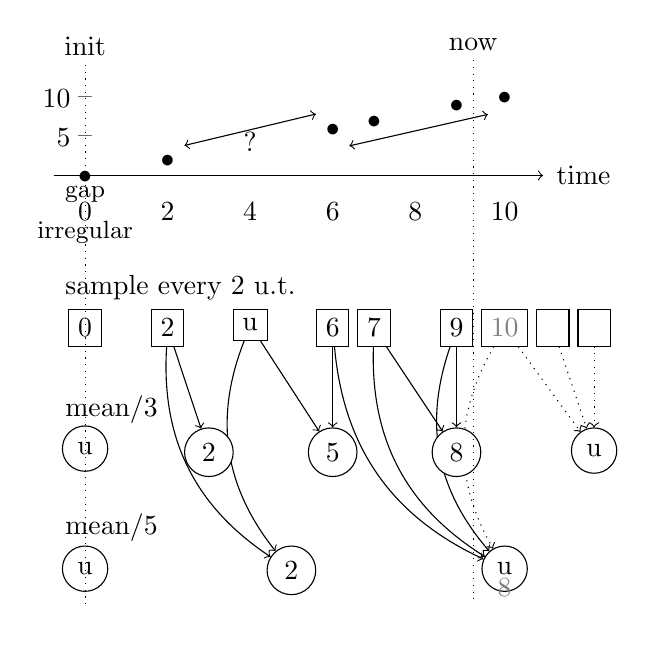
\begin{tikzpicture}

  \node[node distance=1mm] (0) {0};
  \node[node distance=1mm] (-1) [left=of 0]{\phantom{9}};
  \node[node distance=1mm] (1) [right=of 0] {\phantom{1}};
  \node[node distance=1mm] (2) [right=of 1] {2};
  \node[node distance=1mm] (3) [right=of 2] {\phantom{3}};
  \node[node distance=1mm] (4) [right=of 3] {4};
  \node[node distance=1mm] (5) [right=of 4] {\phantom{5}};
  \node[node distance=1mm] (6) [right=of 5] {6};
  \node[node distance=1mm] (7) [right=of 6] {\phantom{7}};
  \node[node distance=1mm] (8) [right=of 7] {8};
  \node[node distance=1mm] (9) [right=of 8] {\phantom{9}};
  \node[node distance=1mm] (10) [right=of 9] {10};
  \node[node distance=1mm] (11) [right=of 10] {\phantom{9}};
  \node[node distance=1mm] (12) [right=of 11] {\phantom{9}};


  \node [above=0 mm of 0] {$\bullet$}; 
  \node [above=2 mm of 2] (v2) {$\bullet$}; 
  \node [above=4 mm of 4] {?}; 
  \node [above=6 mm of 6] (v6) {$\bullet$}; 
  \node [above=7 mm of 7] {$\bullet$}; 
  \node [above=9 mm of 9] {$\bullet$}; 
  \node [above=10 mm of 10] (v10) {$\bullet$}; 


  \node[rectangle,draw] (s0) [below=of 0] {0};
  \node[rectangle,draw] (s2) [below=of 2] {2};
  \node[rectangle,draw] (s4) [below=of 4] {u};
  \node[rectangle,draw] (s6) [below=of 6] {6};
  \node[rectangle,draw] (s7) [below=of 7] {7};
  \node[rectangle,draw] (s9) [below=of 9] {9};
  \node[rectangle,draw] (s10) [below=of 10] {\color{gray}10};
  \node[rectangle,draw] (s11) [below=of 11] {\phantom{9}};
  \node[rectangle,draw] (s12) [below=of 12] {\phantom{9}};


  \draw[<->] (v2.north east) to (v6.north west)
  node [above,sloped,midway] {\small gap};

  \draw[<->] (v6.south east) to (v10.south west)
  node [below,sloped,midway] {\small irregular};

  
  %rd: 5s |inf| mean
  \node [circle,draw] (rd50) [below=4cm of 0] {u};
  \node [circle,draw] (rd55) [below=4cm of 5] {2};
  \node [circle,draw] (rd510) [below=4cm of 10] {u};
  \node [below=4.3cm of 10] {\color{gray}8};
 
  \draw[->,bend right] (s4) to (rd55);
  \draw[->,bend right] (s2) to (rd55);

  \draw[->,dotted,bend right] (s10) to (rd510);
  \draw[->,bend right] (s9) to (rd510);
  \draw[->,bend right] (s7) to (rd510);
  \draw[->,bend right] (s6) to (rd510);

  
  %rd: 3s |inf| mean
  \node [circle,draw] (rd30) [below=of s0] {u};
  \node [circle,draw,fill=white] (rd33) [below=2.5cm of 3] {2};
  \node [circle,draw,fill=white] (rd36) [below=2.5cm of 6] {5};
  \node [circle,draw,fill=white] (rd39) [below=2.5cm of 9] {8};
  \node [circle,draw] (rd312) [below=2.5cm of 12] {u};

  \draw[->] (s2) to (rd33);

  \draw[->] (s6) to (rd36);
  \draw[->] (s4) to (rd36);

  \draw[->] (s9) to (rd39);
  \draw[->] (s7) to (rd39);

  \draw[->,dotted] (s12) to (rd312);
  \draw[->,dotted] (s11) to (rd312);
  \draw[->,dotted] (s10) to (rd312);



  %eixos
  \node (et0) [above=1mm of -1] {};
  \node (et12) [above=1mm of 11] {};
  \node [right=-2mm of et12] {time};
  \draw[->] (et0) to (et12);
  \node (y5) [above=5mm of 0] {--};
  \node [left=-1.5mm of y5] {5};
  \node (y10) [above=10mm of 0] {--};
  \node [left=-1.5mm of y10] {10};

  \node (inici) [above=3.1cm of s0] {init};
  \node (inici2) [below=3.3cm of s0] {};
  \draw[-,dotted] (inici) to (inici2);

  \node (fi) [above=3.4cm of s9.east] {now};
  \node (fi2) [below=3.5cm of s9.east] {};
  \draw[-,dotted] (fi) to (fi2);


  % \node (fut) [below right=1mm and 1mm of fi] {future};
  % \draw[->] (fut.south west) to (fut.south east);

  % \node (pas) [below left=1mm and 1mm of fi] {past};
  % \draw[->] (pas.south east) to (pas.south west);

  \node [above=0cm of s0] {\makebox[0.5cm][l]{sample every 2 u.t.}};
  \node [below=0.5cm of s0] {\makebox[0.5cm][l]{mean/3}};
  \node [below=2cm of s0] {\makebox[0.5cm][l]{mean/5}};

\end{tikzpicture}



%%% Local Variables:
%%% TeX-master: "../main"
%%% ispell-local-dictionary: "british"
%%% End:

%   \caption{Multiresolution snapshot diagram with irregular sampling}
%   \label{fig:mtsms:sequence-irregular}
% \end{figure}



At the bottom of Figure~\ref{fig:mtsms:sequence} there is a diagram
showing the multiresolution action. The first row shows the numerical
time series' values corresponding to the above plot; the time series
is sampled every one unit of time. The second and the third row show a
particular schema of a multiresolution database consisting in two time
resolutions for the time series: one computes the mean of the sampled
values every three u.t.\ and the other computes the mean every five
u.t. In this example, computing the mean acts as selecting information
by aggregate statistics. All data stored before zero time is unknown
(\emph{u}) as has not been acquired. For the future values it is also
marked as \emph{u} until time advances.

The arrows of the figure show that every three sampled values a mean
is stored and, independently, every five values another mean is
stored. For the future values, dashed arrows show that if time
advances one u.t.\ then value 10 is sampled and the mean for time 10
can be computed resulting 8 but not yet the mean for time 12.

% Fig.~\ref{fig:mtsms:sequence-irregular} is essentially the same but
% showing two possible monitoring irregularities: a gap and a time
% disruption. In other words, we want to sample the time series every 2
% u.t.\ but first for some reason it can not be done in time 4 and
% second the sampling clock is disrupted and samples are done in time 7
% and 9 instead of 8. The resulting stored time schema is the same: on
% time resolution every 3 u.t.\ and the other every 5 u.t.; that is,
% without time disruptions. The resulting stored values are computed
% from the known sampled values, some coincide with
% fig.~\ref{fig:mtsms:sequence} whereas some differ specially in the
% gap. A better function than mean would solve this, we extend this
% further in section~\ref{sec:model:interpolador}.



%%% Local Variables:
%%% TeX-master: "main"
%%% ispell-local-dictionary: "british"
%%% End:

%  LocalWords:  multiresolution TSMS MTSMS



\section{Formalització dels models}
\begin{frame}{Formalització dels models}

  \begin{enumerate}
  \item Sistemes de gestió de sèries temporals (SGST)
  \item Exemple de multiresolució
  \item Sistemes de gestió de sèries temporals multiresolució (SGSTM)
  \end{enumerate}

\end{frame}

\chapter{Model SGST}
\label{cap:model:sgst}


En aquest capítol es defineix un model per als sistemes de gestió de
bases de dades per a sèries temporals (SGST). Aquest model
s'estructura en base a dos objectes principals, mesures i sèries temporals.
Ambdós tenen un atribut de temps, el qual requereix un tractament
adequat. El model de SGST es dissenya en tres parts.

\begin{itemize}

\item Primer, es defineix el model d'estructura de les dades, és a
  dir, la forma com es descriuen les mesures i les sèries temporals.  

\item Segon, es defineix el model d'operacions sobre les dades, és a
  dir, els operadors bàsics que permeten modelar el comportament i la
  manipulació de les sèries temporals.

\item Tercer, es descriuen propietats de les sèries
  temporals. Les sèries temporals adquireixen propietats
  variades depenent del context on s'apliquin.

\end{itemize}





\section{Model estructural de dades}

Una sèrie temporal és una relació de temps i valors. A cada parella
temps-valor l'anomenem mesura. Així doncs, una sèrie temporal és un
conjunt de mesures. 


En el nostre cas concret, una mesura es correspon amb un valor mesurat
en un instant de temps i una sèrie temporal esdevé una co\l.lecció de
mesures.





\subsection{Temps}
\label{sec:sgst:temps}

El temps és la variable que ens permet ordenar les mesures.  A tal
efecte, si denominem $T$ el domini del temps, els seus membres
presenten una relació d'ordre total. $T$ pot ser tant un conjunt finit
com infinit i normalment serà un conjunt tancat %(compactificat?)
per a poder incloure les mesures indefinides (v.\
\autoref{def:model:mesura_indefinida}) com a límits.

Per tal de facilitar la comprensió, en el document utilitzarem el
conjunt de reals com a conjunt pels temps. Representarem el conjunt
$T$ amb el conjunt estès de nombres reals $\bar{\R{}} \in
\R{} \cup
\{+\infty,-\infty\}$, \parencite{wiki:extendedreal,cantrell:extendedreal},
també anomenat recta real acabada, el qual és un conjunt tancat.

El conjunt estès de nombres reals té dos punts límits corresponents al
valor impropi infinit, aleshores en notació d'interval el conjunt $T$
es pot escriure com $\bar{\R{}} \in [-\infty,+\infty]$. En referència
amb el conjunt dels nombres reals $\R{}$, les relacions d'ordre i
algunes operacions aritmètiques s'estenen al conjunt $\bar{\R{}}$,
\cite{cantrell:extendedreal}.  Algunes expressions esdevenen
indefinides (p.ex.\ $0/0$) i altres depenen del context, com és el cas
de l'expressió indeterminada $0 \times \infty$ que per exemple en la
teoria de la mesura habitualment es defineix com $0 \times \infty =
0$, \cite{wiki:extendedreal}.


El conjunt dels reals és un espai mètric ja que té definida una funció
distància (o mètrica), com per exemple la distància euclidiana. Com a
conseqüència, ens permet distingir entre instants de temps (els
elements del conjunt) i durades (la mètrica). Observant els instants
de temps com a punts en la recta real, les durades com a segments de
la recta real i especificant un instant de temps com a marc de
referència, es pot definir el temps com a sistema de
coordenades \parencite{iep:time-supplement,wiki:coordinate,kopetz11:realtime}. A
continuació definim el temps de manera que puguem ordenar
esdeveniments, mesurar durades d'esdeveniments i establir quan
esdevenen; és una aproximació ingènua sense abastar detalls complicats
del concepte temps \parencite{iep:time}.

\todo{s'hauria de dir que kopetz també en fa una definició similar}



\begin{definition}[Temps]
  \label{def:model:temps}
  Siguin $t^i_i$ i $t^i_j$ dos instants de temps amb el mateix $t^R$
  com a marc de referència, definim la quantitat de temps o la durada
  $t^d$ com un valor $t^d \in\bar{\R{}}$ que mesura la distància en
  unitats de temps entre dos instants de temps $t^d = d(t^i_i,t^i_j)$
  a on $d$ és la mètrica del conjunt $T$. En el cas que els instants
  de temps es defineixin com a reals, $t^i_i , t^i_j \in \bar{\R{}}$,
  aleshores $t^d = t^i_i - t^i_j$.

  Sigui $T$ el domini del temps, definim un instant de temps $I$ com
  un element del conjunt $I \in T$. Així, un instant de temps és
  l'etiqueta d'un punt en la línia temporal. Seguint la definició de
  sistema de coordenades i prenent els nombres reals com a domini del
  temps, sigui $t^{R}$ un instant de temps marc de referència,
  aleshores els instants de temps es defineixen com un valor $t^i
  \in\bar{\R{}}$ que indica la distància de temps amb signe respecte a
  l'instant de temps de referència $t^i= d(t^{R},I)$ a on $d$ és la
  mètrica del conjunt $T$.
\end{definition}

En resum, els instants de temps es poden veure com una seqüència de
valors reals que indiquen esdeveniments amb ordre clarament definit i
entre dos instants de temps sempre hi ha una durada. Expressarem tant
els instants de temps com les durades amb un real que té unitats de
temps. Aquestes unitats són 'segons' en sistema internacional.

% El marc de referència és un instant de temps que permet definir
% unívocament la posició de qualsevol altre instant de temps en un
% sistema de coordenades.



\subsubsection{Estàndards de temps}

Els estàndards de temps especifiquen com s'ha de mesurar el pas del
temps i com s'han d'assenyalar els instants de temps.
\textcite{allen:timescales} recull diferents estàndards de temps
que existeixen, dels quals a continuació comentem els més habituals.

Actualment l'estàndard de temps habitual per mesurar el pas del temps
és el Temps Atòmic Internacional (TAI), del qual se'n deriva un altre
estàndard més conegut que és el Temps Universal Coordinat (UTC).
Ambdós estàndards assenyalen el instants de temps segons el calendari
Gregorià i el calendari julià. Actualment, de forma genèrica s'utilitza
UTC per a sincronitzar rellotges tot i que en el futur es podria
canviar per un nou estàndard, el Temps Internacional (TI), el qual
també es base en el TAI.

El calendari julià utilitza un estàndard de comptar el temps com a
nombre de dies que han passat des d'una data concreta, la qual
s'anomena època. L'època es correspon amb el concepte d'instant de
temps marc de referència de la \autoref{def:model:temps}. Per defecte
l'època se situa a l'inici del Període Julià tot i que també se solen
utilitzar altres dates assenyalades.

Un altre estàndard semblant al julià és l'Hora POSIX o Hora Unix, el
qual compta el nombre de segons des de l'1 de gener de 1970 basant-se
en el les mesures d'UTC. L'Hora Unix és l'estàndard de temps habitual
en els sistemes operatius de la família Unix. No obstant, aquest
estàndard presenta un problema d'ambigüitat a causa que no té no té en
compte els segons addicionals d'UTC.





\subsubsection{Calendari}

Un cas particular del temps és el calendari. Els calendaris són
definicions pel domini temps que consisteixen en noms per als punts de
la línia de temps i regles per establir la durada entre ells per tal
de que el temps tingui certa relació amb la rotació de la Terra. A
l'apartat anterior hem definit el domini temps de manera general
amb el conjunt de reals, els quals exemplifiquen més clarament el
concepte de sistema de coordenades de temps absolut.

\textcite{dreyer94} situen els calendaris i les seves operacions com a
essencials en els SGST. Tanmateix, pot no ser necessari modelar les
dates i regles de calendari en el model de temps. Els calendaris es
poden observar com a noms que fan referència a instants de temps
quantificables, com els de la \autoref{def:model:temps}. Aleshores,
només cal una eina que sigui capaç de convertir els noms de calendari
a instants de temps.

El fet de que un calendari sigui més o menys complicat no afecta al
model de SGST, sols té incidència en les funcions de conversió
d'instant de temps a calendari i viceversa. Tampoc afecta que els
calendaris siguin ambigus (p.ex.\ dos noms per al mateix instant o
instants sense nom) o que continguin propietats impredictibles (p.ex.\
cas dels segons addicionals en UTC) ja que aquests casos es
corresponen amb la bona definició dels sistemes de calendari.

Així doncs, els calendaris en el model de SGST es poden implementar
com una extensió del model de temps. El tipus de dades ordinal de
calendari Gregorià implementat per
\textcite[cap.~16]{date02:_tempor_data_relat_model} pot servir com a
guia per a la implementació dels calendaris en els SGST.




\subsection{Valor}
\label{sec:sgst:valor}

\todo{T: refer tota la secció}

El \gls{terme:SGBDR:valor} és qualsevol element que és d'un
\gls{terme:SGBDR:tipus}; és a dir, un objecte que
pertany a un determinat conjunt de valors i que té associat les
operacions que s'hi poden aplicar. Exemples de tipus de dades són els
enters, els reals, les cadenes de text i les estructures de dades com
vectors, llistes o \glspl{terme:SGBDR:relacio}.  

\todo{Exemplificar més amb tipus que tenen valors i operacions que se'ls poden aplicar}

%\todo{potser citar que el valor es tracta de manera semblant a l'extensió del model objecte-relacional?}

El model de dades dels valors ha d'incloure una dada que defineixi el
valor indefinit. Més endavant a la
definició~\ref{def:model:mesura_valor_indefinit} es detallen les
propietats de les mesures amb valor indefinit. Seguint l'exemple amb
els reals, el valor indefinit es defineix amb el valor impropi infinit
del conjunt dels reals estès
projectivament, \parencite{cantrell:projectivelyextendedreal},
$\R{}^*\in\R{} \cup \{\infty\}$.


En aquest exemple amb reals, el valor és un escalar però fàcilment es
pot estendre el concepte a valors multivaluats ${\R{}^*}^n$ que
representin una co\l.lecció de valors mesurats en el mateix instant de
temps, tal i com fa per exemple \textcite{assfalg08:thesis}.







\subsection{Mesura}\label{sec:model:mesura} 

Una mesura està formada per la parella de temps i valor.

\begin{definition}[Mesura]
  \label{def:model:mesura}
  Definim \emph{mesura} com el tuple $(t,v)$, en el que $v$ és el
  valor de la mesura i $t$ és l'instant de temps en que s'ha pres
  aquesta mesura.
\end{definition}


Donada una mesura $m=(t,v)$ escriurem $V(m)$ per referir-nos a $v$ i
$T(m)$ per referir-nos a $t$.

L'instant de temps de les mesures indueix una relació d'ordre entre
les mesures.
\begin{definition}[Relació d'ordre]\todo{dir-li temporal, perquè sinó després $m\in S$ queda com $m\in^tS$. Arreglar-ho a les definicions de pertinença }
  \label{def:model:mesura-relacio-ordre}
  Sigui $m=(t_m,v_m)$ i $n=(t_n,v_n)$, direm que l'ordre de la mesura
  $m$ és major o igual que $n$, $m\geq n$, si i solament si $t_m\geq
  t_n$.
\end{definition}\todo{també hem de definir l'ordre parcial $m<n$ per la definició de pertinença no temporal?}


En les definicions de temps i valor s'han estès els conjunts amb
valors impropis, concretament s'ha exemplificat amb el conjunt estès
de nombres reals afí $\bar{\R{}} \in \R{} \cup
\{+\infty,-\infty\}$ i amb el projectiu $\R{}^*\in\R{}
\cup\{\infty\}$,
\parencite{cantrell:extendedreal,cantrell:projectivelyextendedreal}. Aquesta
extensió amb l'element impropi infinit ($\infty$) dóna com a resultat
unes mesures impròpies que anomenarem mesura de valor indefinit i
mesura indefinida.\todo{potser s'hauria de dir de no confondre el valor indefinit amb l'absència de valor; és a dir que en una sèrie temporal les mesures que no hi són, són absents (no s'han pres) i les mesures de valor indefinit s'han pres però tenien un valor erroni o desconegut (més a la secció de patologies).} 

\begin{definition}[Mesura de valor indefinit]
  \label{def:model:mesura_valor_indefinit}
  Definim \emph{mesura de valor indefinit} com el tuple $(t,v)$, en el
  que el valor és $v=\infty$ i l'instant de temps és
  $t\in\bar{\R{}}$.
\end{definition}

\begin{definition}[Mesura indefinida]
  \label{def:model:mesura_indefinida}
  Definim \emph{mesura indefinida} com el tuple $(t,v)$, en el que el
  valor és $v\in\R{}^*$ i l'instant de temps és
  $t\in\{+\infty,-\infty\}$.
\end{definition}

Així doncs, donada una mesura $m$, s'anota la mesura de valor
indefinit com $m=(t,\infty)$ i les mesures indefinides com
$m=(+\infty,v)$ per la positiva i $m=(-\infty,v)$ per la negativa, les
quals normalment s'anotaran també amb valor indefinit:
$m=(+\infty,\infty)$ i $m=(-\infty,\infty)$ respectivament.


Les mesures de valor indefinit es podran utilitzar en aquells casos en
els que el valor de la mesura és desconegut. Els valors desconeguts
són aquells valors que no existeixen (es desconeixen, \emph{missing
  data} ) o que s'ignoren (es descarten, \emph{censoring} o
\emph{truncation}). Els valors que no existeixen prenen el valor
desconegut en el moment de la mesura, en canvi els valors descartats
són marcats com a desconeguts després d'un processament de les dades.

Nota: en alguns sistemes es distingeix entre valors infinits
($\infty$) i valors indefinits (NaN, \emph{not a number}),
\cite{wiki:ieee754}. Aquest no és el cas de les definicions de mesures
indefinides presents.







\subsection{Sèrie temporal}
\label{sec:model:serietemporal}

Les sèries temporals són seqüències de mesures ordenades en el temps.
Tradicionalment s'anomenen sèries temporals tot i que alguns autors les anomenen
seqüències temporals, per exemple a \cite{last:hetland}.  Les sèries
temporals són mesures del mateix fenomen i com a conseqüència el tipus
dels valors de les sèries temporals és homogeni.


\begin{definition}[Sèrie temporal]
  \label{def:serie_temporal}
  Una sèrie temporal $S$ és un conjunt de mesures
  $S=\{m_0,\ldots,m_k\}$ sense temps repetits en la qual
  $\forall i,j: i\leq k, j\leq k, i\neq j : T(m_i)\neq T(m_j)$.
\end{definition}

Per ser un conjunt, les sèries temporals tenen mesura de cardinalitat.
\begin{definition}[Cardinal]
  Sigui $S=\{m_0,\ldots,m_k\}$ una sèrie temporal, definim el nombre
  de mesures que conté la sèrie temporal com el cardinal del conjunt
  $|S|=k+1$. Una sèrie temporal sense mesures és la sèrie temporal
  buida $S_\emptyset= \emptyset = \{\}$, és a dir que no té cap element
  $|S_\emptyset|=0$.
\end{definition}



 
\subsubsection{Formes d'una sèrie temporal}

Una sèrie temporal pot tenir formes diferents segons com s'expressi.
A continuació diferenciem entre tres formes possibles d'una sèrie
temporal: canònica, multivaluada i doble.


La forma bàsica d'una sèrie temporal és la de parelles de temps i
valor a la qual anomenem forma canònica.
\begin{definition}[Forma canònica]
  Sigui $S = \{ m_0, m_1 , \dotsc, m_k \}$ una sèrie temporal,
  s'escriu com $S =  \{
  (t_0,v_0), (t_1,v_1), \dotsc, (t_k,v_k)\}$; és
  a dir com a parelles de temps i valor. A aquesta
  forma l'anomenem canònica.
\end{definition}


Les sèries temporals poden mesurar alhora més d'un fenomen quan
aquests comparteixen els instants de temps de mesura. Aquestes sèries
temporals tenen forma de sèrie temporal multivaluada.

\begin{definition}[Sèrie temporal multivaluada]
  Anomenem sèrie temporal multivaluada a una sèrie temporal que té més
  d'un atribut de valors.  Sigui $S = \{ m_0, m_1 , \dotsc, m_k \}$
  una sèrie temporal és multivaluada si cada mesura $m_i$ és un tuple
  $m_i=(t,v_1,v_2,\dotsc,v_n)$ a on $t$ és un instant de temps i
  $v_1$, $v_2$, \dots, $v_n$ són valors. 

  Una sèrie temporal multivaluada es pot escriure en forma canònica de
  parelles $(t,v)$. És a dir, la sèrie temporal multivaluada en
  forma canònica té mesures $m_i$ com a tuples
  $m_i=(t,(v_1,v_2,\dotsc,v_n))$
\end{definition}

La forma canònica s'utilitza per a generalitzar les sèries temporals
multivaluades en les operacions on el valor multivaluat no és
rellevant. En altres operacions, per exemple la selecció o la junció,
el multivalor és rellevant per treballar-hi o perquè el resultat és
una sèrie temporals multivaluada. 



Hi ha una forma no habitual de les sèries temporals que es dóna quan
tenen dos atributs de temps i a la qual anomenem forma doble.

\begin{definition}[Sèrie temporal doble]
  \label{def:sgst:st-doble}
  Anomenem sèrie temporal doble a una sèrie temporal que té dos
  atributs de temps i dos atributs de valors. Sigui $S =\{m_0, \dotsc,
  m_k\}$ una sèrie temporal és doble si cada mesura $m_i$ és un tuple
  $m_i=(t_1,v_1,t_2,v_2)$ a on $t_1$ i $t_2$ són instants de temps i
  $v_1$ i $v_2$ són valors. De la mateixa manera, a aquesta mesura
  $m_i$ l'anomenem mesura doble.  Una sèrie temporal doble no té dues
  parelles de temps repetides $|\{(t_1,t_2) | t_1,t_2\in S\}| = |S|$.
\end{definition}

La sèrie temporal doble prové d'un producte de dues sèries
temporals. Està pensada com a càlcul intermedi d'altres operacions com
per exemple la junció o el mapatge. 
% La seva forma canònica es
% correspondria de manera semblant a l'exemple de la
% \autoref{fig:model:serietemporal:serietemporal}.









\subsubsection{Relació sèrie temporal}

Una sèrie temporal s'expressa com un conjunt i com a tal és
susceptible d'aplicar-hi els conceptes del model relacional dels
SGBD. A continuació, el que s'ha descrit a l'apartat anterior es torna
a expressar seguint el concepte de relació.


Per ser un conjunt de mesures, s'observa una sèrie temporal com una
relació de grau dos a on la capçalera conté els atributs temps i
valor. Ambdós atributs tenen els dominis de temps i valor descrits a
les seccions \ref{def:model:temps} i \ref{sec:sgst:valor}, com per
exemple el tipus de dades 'reals estesos'. Les relacions de sèries
temporals inclou algunes restriccions més que les relacions:

\begin{itemize}
\item Els temps no poden estar repetits: (\emph{key restriction \{t\}})
\item L'atribut de valor ha de contenir el mateix tipus d'objecte i ha
  d'estar associat al mateix fenomen o fenòmens.
\end{itemize}

Els temps no repetits indueixen un ordre temporal a les sèries
temporals. Tot i així, les relacions, per ser conjunts, conserven la
no definció d'un ordre dels elements. En el model relacional no hi ha
ordre ni en les tuples ni en els atributs a diferència de les
relacions matemàtiques que tenen un ordre d'esquerra a
dreta \parencite[sec.\ 5.3]{date:introduction}.


%\subsubsection{Possibles representacions}

A l'apartat anterior s'han descrit diverses formes d'una sèrie
temporal.  A continuació atenem a les possibles representacions com a
relació d'una sèrie temporal segons les formes que tinguin.

% Com a relació seguint el concepte de possibles
% representacions proposat per \textcite[cap.~5]{date:introduction} ?
% i les formes normals de les relacions [Date]?



\begin{definition}[Representació canònica]
  Sigui $S = \{ m_0, m_1 , \dotsc, m_k \}$ una sèrie temporal amb
  domini $\bar{\R{}}$ pels temps i els valors de les mesures,
  representada com a relació s'escriu com $S = ( \{t: \bar{\R{}}, v:
  \bar{\R{}}\}, \{ \{t:t_0,v:v_0\}, \{t:t_1,v:v_1\}, \dotsc,
  \{t:t_k,v:v_k\} \} )$; és a dir com a parella capçalera i conjunt de
  valors certs. A aquesta representació l'anomenem forma canònica.

  Així doncs, sigui $S_{\emptyset} = \{ \}$ una sèrie temporal buida,
  modelada com a relació s'escriu com $S_{\emptyset} = ( \{t:
  \bar{\R{}}, v: \bar{\R{}}\}, \{ \} )$.
\end{definition}


Degut al format esquemàtic de les sèries temporals, en simplifiquem
l'escriptura de la forma canònica com a conjunt de tuples $(t,v)$ a on
$t$ és el temps i $v$ és el valor. Així doncs quan no hi ha dubte
sobre els dominis ni els noms d'atributs, una sèrie temporal es pot
escriure de manera simplificada com a $S = \{ (t_0,v_0), (t_1,v_1),
\dotsc, (t_k,v_k) \}$, la qual es correspon amb la forma canònica de
la sèrie temporal representada com a conjunt.

Tal com s'utilitza en les relacions, les sèries temporals es poden
visualitzar com a taules. La sèrie temporal $S$ i la $S_{\emptyset}$
es visualitzen com a taula a la
\autoref{fig:model:serietemporal:taula}.

\begin{figure}[tp]
  \centering
  \begin{tabular}[c]{|c|c|}
    \multicolumn{2}{c}{$S$} \\ \hline
    $t$  & $v$ \\ \hline
    $t_0$  & $v_0$ \\
    $t_1$  & $v_1$ \\
    $\dots$  & $\dots$ \\ 
    $t_k$  & $v_k$ \\ \hline
  \end{tabular} \qquad
  \begin{tabular}[c]{|c|c|}
    \multicolumn{2}{c}{$S_{\emptyset}$} \\ \hline
    $t$  & $v$ \\ \hline
      &  \\ \hline
  \end{tabular}
  \caption{Visualització com a taula d'una sèrie temporal}
  \label{fig:model:serietemporal:taula}
\end{figure}




\begin{definition}[Representació multivaluada]
  La representació com a relació d'una sèrie temporal multivaluada buida és
  $S_{\emptyset} = ( \{t: \bar{\R{}}, v_1: \bar{\R{}}\,
  v_2: \bar{\R{}}, \dotsc, v_n: \bar{\R{}}\}, \{ \} )$

  Una sèrie temporal multivaluada es pot escriure en forma canònica de
  parelles $(t,v)$. És a dir, la sèrie temporal multivaluada buida en
  representació canònica és $S_{\emptyset} = ( \{t: \bar{\R{}},
  v: V \}, \{ \} )$ a on el domini de l'atribut valor és de tipus
  relació $V = \{ v_1: \bar{\R{}}\, v_2: \bar{\R{}},
  \dotsc, v_n \}$ amb restricció que els valors relació que hi
  pertanyen només poden tenir un tuple $r \in V: |r| = 1$.
\end{definition}

Com ocorre en les relacions, el nom dels atributs d'una sèrie
temporal pot ser decidit per l'usuari. Per exemple una sèrie temporal
multivaluada amb tres atributs amb nom: $S_{\emptyset} = ( \{t:
\bar{\R{}}, \text{temperatura}: \bar{\R{}}\,
\text{consum}: \bar{\R{}}, \text{volum}: \bar{\R{}}\}, \{
\} )$.


Finalment, també representem una sèrie temporal doble en forma de
relació.
\begin{definition}[Representació doble]
  La representació com a relació d'una sèrie temporal doble buida és
  $S_{\emptyset} = ( \{t_1: \bar{\R{}}, v_1: \bar{\R{}}\,
  t_2: \bar{\R{}}, v_2: \bar{\R{}}\}, \{ \} )$.
\end{definition}




\subsection{Exemples}


\begin{example}[Valors reals]
  Sèrie temporal $S_1$ on el temps i els valors pertanyen a
  $\bar{\R{}}$. Conté la mesura de valor 1 en el temps 2, la mesura de
  valor 3 en el temps 2 i la mesura de valor 1 en el temps 6.

En la forma canònica completa s'escriu com $S_1 = ( \{t:
\bar{\R{}}, v: \bar{\R{}}\}, \{ \{t:2,v:1\}, \{t:3,v:3\},
\{t:6,v:1\} \} )$. També es pot escriure de manera simplificada com a
$S_1 = \{ (2,1), (3,3), (6,1) \}$.


La sèrie temporal $S_1$ es visualitza com a taula a la
\autoref{fig:model:serietemporal:real}, a la qual hi afegim una
visualització com diagrama de dispersió amb el temps a l'eix
horitzontal i el valor a l'eix vertical.

\begin{figure}[tp]
  \centering
  \begin{tabular}[c]{|c|c|}
    \multicolumn{2}{c}{$S_1$} \\ \hline
    $t$  & $v$ \\ \hline
    2  & 1 \\
    3  & 3 \\
    6  & 1 \\ \hline
  \end{tabular} \qquad
  \begin{tikzpicture}[baseline=(current bounding box.center)]
    \begin{axis}[
        timeseriesrel,
        title=$S_1$,
        ]
    \addplot[only marks,mark=*,blue] coordinates {
        (2,1)
        (3,3)
        (6,1)
    };
    \end{axis}
   \end{tikzpicture}
  \caption{Taula i gràfic d'una sèrie temporal amb valors reals}
  \label{fig:model:serietemporal:real}
\end{figure}

\end{example}


\begin{example}[Valors caràcters]
  Sèrie temporal $S_2$ on el temps pertany a $\bar{\R{}}$ i els valors
  són caràcters que pertanyen a $C=\{a,b,\dotsc,z,\infty\}$. Conté el
  caràcters $a$, $c$ i $a$ mesurats respectivament en els temps $2$,
  $3$ i $6$.

De manera simplificada s'escriu com $S_2 = \{ (2,a), (3,c), (6,a) \}$.
La sèrie temporal $S_2$ es visualitza com a taula a la
\autoref{fig:model:serietemporal:caracter}, a la qual hi afegim una
visualització com diagrama de dispersió amb el temps a l'eix
horitzontal i el valor a l'eix vertical no continu.

\begin{figure}[tp]
  \centering
  \begin{tabular}[c]{|c|c|}
    \multicolumn{2}{c}{$S_4$} \\ \hline
    $t$  & $v$ \\ \hline
    2  & a \\
    3  & c \\
    6  & a \\ \hline
  \end{tabular} \qquad
  \begin{tikzpicture}[baseline=(current bounding box.center)]
    \begin{axis}[
        timeseriesrel,
        title=$S_4$,
        yticklabels={0,0,a,b,c},
        ]
    \addplot[only marks,mark=*,blue] coordinates {
        (2,1)
        (3,3)
        (6,1)
    };
    \end{axis}
   \end{tikzpicture}
  \caption{Taula i gràfic d'una sèrie temporal amb valors caràcters}
  \label{fig:model:serietemporal:caracter}
\end{figure}

\end{example}



\begin{example}[Sèrie temporal multivaluada]
  Sèrie temporal $S_3$ on el temps pertany a $\bar{\R{}}$ i hi ha tres
  valors on cadascun pertany a $\bar{\R{}}$. En els temps $2$, $3$ i
  $6$ s'ha mesurat a) un atribut \emph{temp} amb valors $1$, $2$ i
  $1$; b) un atribut \emph{cons} amb valors $2$, $1$ i $2$; i c) un
  atribut \emph{vol} amb valors $3$, $0$ i $3$.



En la forma multivaluada s'escriu com %
$S_3 = ( \{t: \bar{\R{}}, \text{ temp}: \bar{\R{}}, \text{
  cons}: \bar{\R{}},\text{ vol}: \bar{\R{}} \}, %
\{%
\{t:2,\text{ temp}:1 , \text{ cons}:2,\text{ vol}:3 \}, %
\{t:3,\text{ temp}:2 , \text{ cons}:1,\text{ vol}:0 \}, %
\{t:6,\text{ temp}:1 , \text{ cons}:2,\text{ vol}:3 \} %
\} )$. També es pot escriure de manera simplificada com a $S_{3} = (
(t,\text{ temp},\text{ cons},\text{ vol}),\{ (2,1,2,3), (3,2,1,0),
(6,1,2,3) \})$.

La forma canònica és una sèrie temporal amb tuples $(t,v)$, és a dir
\begin{align*}
  S^C_{3} &= ( \{t: \bar{\R{}}, v: \{ \text{ temps}:
  \bar{\R{}}, \text{ cons}: \bar{\R{}},\text{ vol}:
  \bar{\R{}},\} \}, \{ \\
  & \{t:2, v: ( \{ \text{ temp}: \bar{\R{}}, \text{ cons}:
  \bar{\R{}},\text{ vol}: \bar{\R{}},\}, \{ \text{ temp}:1
  ,  \text{ cons}:2,\text{ vol}:3 \}\} ), \\
 & \{t:3, v: ( \{ \text{ temp}: \bar{\R{}}, \text{ cons}:
  \bar{\R{}},\text{ vol}: \bar{\R{}},\}, \{ \text{ temp}:2
  ,  \text{ cons}:1,\text{ vol}:0 \}\} ), \\
 & \{t:6, v: ( \{ \text{ temp}: \bar{\R{}}, \text{ cons}:
  \bar{\R{}},\text{ vol}: \bar{\R{}},\}, \{ \text{ temp}:1
  ,  \text{ cons}:2,\text{ vol}:3 \}\} ) \\
  \} )
\end{align*}


La sèrie temporal $S_3$ i la seva forma canònica es visualitzen com a
taula a la \autoref{fig:model:serietemporal:caracter}, a la qual hi
afegim una visualització com diagrama de dispersió amb el temps a
l'eix horitzontal i els valor a l'eix vertical cadascun amb color
diferent.


\begin{figure}[tp]
  \centering
  \begin{tabular}[tp]{|c|c|c|c|}
   \multicolumn{4}{c}{$S_3$} \\ \hline
    $t$  & temp & cons & vol \\ \hline
    2  & 1 & 2 & 3 \\
    3  & 2 & 1 & 0 \\
    6 & 1 & 2 & 3 \\ \hline
  \end{tabular}\qquad
  \begin{tabular}{|c|ccc|}
    \multicolumn{4}{c}{$S_3^c$} \\ \hline
    \multirow{2}{*}{$t$}  & \multicolumn{3}{c|}{$v$} \\ \cline{2-4}
       & temp & cons & vol \\ \hline
    2  & 1 & 2 & 3 \\
    3  & 2 & 1 & 0 \\
    6  & 1 & 2 & 3 \\ \hline
  \end{tabular} 
  \begin{tikzpicture}[baseline=(current bounding box.center)]
    \begin{axis}[
        timeseriesrel,
        title=$S_3$,
        legend columns = 4,
        every axis legend/.append style={
          at={(1,-0.1)},
          anchor=north east,
          draw = none},
        ]
    \addplot[only marks,mark=*,blue] coordinates {
        (2,1)
        (3,2)
        (6,1)
    };
    \addplot[only marks,mark=*,red] coordinates {
        (2,2)
        (3,1)
        (6,2)
    };
    \addplot[only marks,mark=*,green] coordinates {
        (2,3)
        (3,0)
        (6,3)
    };
    \legend{temp,cons,vol}
    \end{axis}
  \end{tikzpicture}
  %El gràfic d'una multivaluada: es poden pintar dos eixos verticals quan les diferències d'escala siguin molt grans.
  \caption{Taula d'una sèrie temporal multivaluada}
  \label{fig:model:serietemporal:multivaluada}
\end{figure}


\end{example}



\begin{example}[Valors vectors]
  Sèrie temporal $S_4$ on el temps pertany a $\bar{\R{}}$ i el valor
  pertany a $\bar{\R{}}^3$; és a dir és un vector representat amb un
  tuple. Conté el valor $(1,2,3)$ en el temps $2$, el valor $(3,4,5)$
  en el temps $4$ i el valor $(1,2,3)$ en el temps $6$.

De manera simplificada s'escriu com $S_4 = \{ (2,(1,2,3)),
(3,(3,4,5)), (6,(1,2,3)) \}$ i es visualitza com a taula i com a
gràfic a la \autoref{fig:model:serietemporal:vector}.

\begin{figure}[tp]
  \centering
  \begin{tabular}{|c|c|}
    \multicolumn{2}{c}{$S_4$} \\ \hline
    $t$  & $v$ \\ \hline
    2  & (1,2,3) \\
    4  & (3,4,5) \\
    6  & (1,2,3) \\ \hline
  \end{tabular} \qquad
  \begin{tikzpicture}[baseline=(current bounding box.center)]
\begin{axis}[
        timeseriesrel,
        nodes near coords,
        title=$S_4$,
        yticklabels={},
        axis y line=none,
        ]
        \addplot+[only marks,mark=none,blue, point meta=explicit symbolic]
        coordinates {
          (2,0)  [\rotatebox{45}{(1,2,3)}]
          (4,0)  [\rotatebox{45}{(3,4,5)}]
          (5,1)  [\mbox{}]
          (6,0) [\rotatebox{45}{(1,2,3)}]
        };
      \end{axis}
    \end{tikzpicture}
    \caption{Taula d'una sèrie temporal amb valors vectors}
  \label{fig:model:serietemporal:vector}
\end{figure}



S'observa que una sèrie temporal amb valors vectors és diferent d'una
sèrie temporal multivaluada. El domini de la primera són vectors i el
de la segona són relacions d'un sol tuple en els que es pot operar
cada atribut per separat. En els vectors de forma general no es poden
operar cada component per separat sinó que formen una unitat
semàntica. Aquesta diferència de significat prové de si es considera
que es mesuren vectors o atributs diferents, el qual s'observa en la
visualització: el gràfic d'un vector és un espai $R^n$ en canvi el
gràfic d'una sèrie temporal multivaluada és un multigràfic, un gràfic
per a cada atribut.

\end{example}


\begin{example}[Valors sèrie temporal]\label{par:model:exemple-relvalues}
  Sèrie temporal $S_5$ on el temps pertany a $\bar{\R{}}$ i el valor
  és una sèrie temporal del mateix format que en l'exemple 1. Conté
  els tuples de $S_1$ com a valors en el temps $1$ i $2$.

De manera simplificada s'escriu com $S_5 = \{ (1,\{ (2,1), (3,3),
(6,1) \}), (2,\{ (2,1),$ $(3,3),$ $(6,1) \}) \}$ i es visualitza com a
taula a la \autoref{fig:model:serietemporal:serietemporal}.


\begin{figure}[tp]
  \centering
  \begin{tabular}{|c|c|}
    \multicolumn{2}{c}{$S_5$} \\ \hline
    $t$  & $v$ \\ \hline
    1 &   
       \begin{tabular}{|c|c|}
         \hline
         $t$  & $v$ \\ \hline
         2  & 1 \\
         3  & 3 \\
         6  & 1 \\ \hline
       \end{tabular} \\ \hline
    2 & 
       \begin{tabular}{|c|c|}
         \hline
         $t$  & $v$ \\ \hline
         2  & 1 \\
         3  & 3 \\
         6  & 1 \\ \hline
       \end{tabular} \\ \hline
  \end{tabular}
  \caption{Taula d'una sèrie temporal amb valors sèrie temporal}
  \label{fig:model:serietemporal:serietemporal}
\end{figure}

S'observa que la capçalera de $S_5$ és $\{t:\bar{\R{}},v:
\{t:\bar{\R{}},v:\bar{\R{}}\}\}$. És a dir, el valor és
una altra relació, com es descriu per \textcite[sec.\
5.3]{date:introduction}, a on el temps i el valor pertanyen a
$\bar{\R{}}$. Per tant, el valor de $S_5$ és de tipus sèrie
temporal amb valors reals. Tot i així, aquest és un valor especial i
si es desplega la relació s'obté una sèrie temporal doble amb
capçalera $\{t^1,t^2,v\}$.

% Cal insistir que \emph{tots} el valors de $S_5$ han de pertànyer al
% mateix domini \parencite[sec.\ 5.4]{date:introduction}, el qual és
% $\{temps:\bar{\R{}},valor:\bar{\R{}}\}$.


\end{example}




















%%% Local Variables:
%%% TeX-master: "main"
%%% End:







% LocalWords:  SGST multivaluada

\chapter{Model SGSTM}
\label{cap:model:sgstm}

En aquest capítol es defineix un \glsdispsec{not:sgstm}{model dels
  sistemes de gestió de bases de dades per a sèries temporals
  multiresolució (SGSTM)}. Aquest model s'estructura en un objecte
principal que són les sèries temporals multiresolució, les quals es
defineixen com a conjunts de subsèries temporals resolució formades
per discs i buffers. El model es dissenya en tres parts.

\begin{itemize}
\item Primer, es defineix el model d'estructura de les dades, és a
  dir, la forma que prenen els buffers, els discs, les subsèries
  resolució, les sèries temporals multiresolució i les bases de dades
  de sèries temporals multiresolució.

\item Segon, es defineix el model d'operacions sobre les dades, és a
  dir, els operadors bàsics que permeten modelar el comportament i la
  manipulació de bases de dades multiresolució.

\item Tercer, s'expliquen amb més detall les funcions específiques del
  model que permeten agregar diferents atributs de les sèries
  temporals per a obtenir les multiresolucions. Les funcions
  d'agregació d'atributs són requerides pel model però en són
  independents.
\end{itemize}




\section{Model estructural de dades}

Els objectes estructurals principals d'un SGSTM, els quals es
defineixen en aquesta secció, són els següents:
\begin{itemize}
\item Buffer
\item Disc
\item Subsèrie temporal resolució
\item Sèrie temporal multiresolució
\item Base de dades de sèries temporals multiresolució
\end{itemize}

Amb aquest elements definim que en una base de dades per a sèries
temporals multiresolució (BDSTM) hi ha sèries temporals multiresolució
a on cada una és una subsèrie temporal resolució formada per una
relació d'un buffer amb un disc. Aquests objectes tenen molta
correspondència amb les sèries temporals i per tant amb el model de
SGST.


\begin{figure}[tp]
\centering
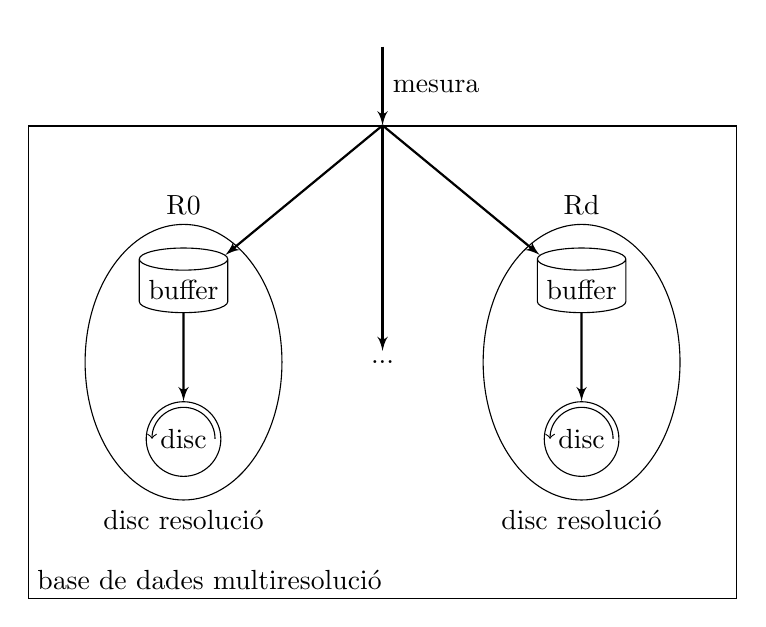
\begin{tikzpicture}
 \tikzset{
        myarrow/.style={->, >=latex',  thick},
      }
      

  \node[rectangle,draw,minimum height=6cm,minimum width=9cm] (m) {};
  \draw[shift=( m.south west)]   
  node[above right] {base de dades multiresolució};


  %discmig
  \node (m.center) (discr1) {...};

  %discr
  
  \node[ellipse,draw,minimum height=3.5cm,minimum width=2.5cm,alias=discr0] [left=of discr1] {};
  \node[above=0cm of discr0.north] {R0};
  \node[below=0cm of discr0] {disc resolució};

  \node[cylinder, draw, shape border rotate=90, aspect=0.25,alias=buffer0] [below=3mm of discr0.north] {buffer};
  \node[circle, draw,alias=disc0]  [above=3mm of discr0.south] {disc} ;
  \draw [->] (disc0.center)++(.4:.4cm) arc(0:180:.4cm);
  \draw[myarrow] (buffer0.bottom) -- (disc0.north);


  %discrd

  \node[ellipse,draw,minimum height=3.5cm,minimum width=2.5cm,alias=discrd] [right=of discr1] {};
  \node[above=0cm of discrd] {Rd};
  \node[below=0cm of discrd] {disc resolució};

  \node[cylinder, draw, shape border rotate=90, aspect=0.25,alias=bufferd] [below=3mm of discrd.north] {buffer};
  \node[circle, draw,alias=discd]  [above=3mm of discrd.south] {disc} ;
  \draw [->] (discd.center)++(.4:.4cm) arc(0:180:.4cm);
  \draw[myarrow] (bufferd.bottom) -- (discd.north);



  %mesura 
  \node[above=1cm of m.north] (m0) {};

  \draw[myarrow] (m0) -- (m.north) 
  node[right,midway] {mesura};

  \draw[myarrow] (m.north) -- (buffer0);
  \draw[myarrow] (m.north) -- (bufferd);
  \draw[myarrow] (m.north) -- (discr1);

\end{tikzpicture}
\caption{Arquitectura d'una BDSTM}
\label{fig:model:bdstm}
\end{figure}


Aquests objectes també permeten definir l'arquitectura d'una BDSTM com
es pot veure a la \autoref{fig:model:bdstm}.  Un SGSTM és una solució
d'emmagatzematge per a sèries temporals a on, resumint, la informació
es distribueix mitjançant diferents resolucions temporals.  Una sèrie
temporal multiresolució és una co\l.lecció de subsèries resolució, les
quals acumulen temporalment mesures en un buffer a on són processades
i finalment emmagatzemades en un disc. El processament de les dades té
per objectiu canviar els intervals de temps entre les mesures per tal
de compactar la informació de les sèries temporals. D'aquesta manera,
les sèries temporals queden emmagatzemades en diferents resolucions
temporals distribuïdes en els discs.

Els discs tenen la mida limitada i només poden contenir un nombre
fixat de mesures. Quan un disc no té més capacitat ha d'eliminar una
mesura. Com a conseqüència una BDSTM té la mida fixada i les sèries
temporals hi queden emmagatzemades a trossos; és a dir com a subsèries
temporals. 


En aquesta secció només es defineixen els conceptes referents a
l'estructura del model. Aquesta estructura, però, requereix uns
operadors específics per a emmagatzemar-hi i consolidar-hi les
mesures, els quals es defineixen a
l'apartat~\ref{sec:model:sgstm-estructurals}. També requereix unes
funcions per a agregar els atributs de les sèries temporals, els quals
es defineixen a l'apartat~\ref{sec:model:agregador}.




\subsection{Buffer}\label{sec:model:buffer}\todo{falta parlar de regularitat de ST}\todo{falta parlar de representació de ST}
\todo{que quedi clar que els buffers deleguen el càlcul a les $f$}

Un buffer és un contenidor d'una sèrie temporal, regular o no regular, que mitjançant una funció permet regularitzar aquesta sèrie temporal amb un període de mostreig constant. A l'acció de regularitzar un interval d'una sèrie temporal l'anomenarem consolidació, al període de mostreig contant l'anomenarem pas de consolidació i a la funció de regularització l'anomenarem agregador d'atributs.

\begin{definition}[Buffer]
  Definim \emph{buffer} com el tuple
  \glsdispdef{not:buffer}{$(S,\tau,\delta,f)$}, en el que
  \glsdispdef{not:sgstm:sb}{$S$} és una sèrie temporal,
  \glsdispdef{not:sgstm:tau}{$\tau$} és el darrer instant de temps de
  consolidació, \glsdispdef{not:sgstm:delta}{$\delta$} és la durada
  del pas de consolidació i \glsdispdef{not:sgstm:f}{$f$} és un
  agregador d'atributs.
\end{definition}

La consolidació d'una sèrie temporal s'inicia en un instant de temps
concret i té lloc a cada pas de consolidació. Amb la finalitat
d'establir els intervals de consolidació de la sèrie temporal, es
defineix un buffer inicial.

\begin{definition}\label{def:model:buffer_buit}
  Definim buffer inicial o buffer buit com el buffer $B_{\emptyset} =
  (\emptyset,t_0, \delta_0, f)$, el qual
  conté una sèrie temporal buida, l'instant de temps inicial de
  consolidació, una durada que indica el pas de consolidació i un
  agregador d'atributs.
\end{definition}

A partir del buffer buit es poden conèixer tots els instants de temps
de consolidació del buffer, els quals seran $t_0+k\delta,
k\in\mathbb{N}$. Aquests instants de temps de consolidació també
defineixen els intervals de temps de consolidació del buffer de la
forma $i=[\tau,\tau+\delta]$. La consolidació de la sèrie temporal $S$
d'un buffer en un interval de temps $i$ dóna com a resultat una mesura
$m=(t,v)$ calculada a partir de l'agregador d'atributs $m = f (S,
i)$. Més endavant a la \autoref{sec:model:agregador} detallem el
concepte d'agregador d'atributs.








\subsection{Disc}\label{sec:model:disc}

Un disc és un contenidor d'una sèrie temporal regular amb un nombre
acotat de mesures. En arribar al nombre màxim de mesures permeses,
cada cop que s'afegeix una mesura nova s'elimina la mesura mínima de
la sèrie temporal.  Així doncs, un disc és semblant a una cua
\emph{First In First Out} (FIFO), a on el primer d'arribar és el
primer de sortir.

\begin{definition}[Disc]
  Definim \emph{disc} com el tuple \glsdispdef{not:disc}{$(S,k)$}, en
  el que \glsdispdef{not:sgstm:sd}{$S$} és una sèrie temporal i
  \glsdispdef{not:sgstm:k}{$k\in\N{}$} és el cardinal màxim de $S$.
\end{definition}

A l'inici, un disc no conté mesures però cal que estigui caracteritzat
pel cardinal màxim. Amb aquesta finalitat es defineix un disc inicial.

\begin{definition}\label{def:model:disc_buit}
  Definim disc inicial o disc buit com el disc $D_{\emptyset} =
  (\emptyset,k)$, el qual conté una sèrie temporal buida i el cardinal
  màxim que podrà prendre $S$.
\end{definition}




\subsection{Subsèrie resolució}\label{sec:model:subserie-resolucio}

Una subsèrie temporal resolució és una parella de disc i buffer. En el
buffer hi ha la part d'una sèrie temporal a regularitzar i en el disc
hi ha l'altra part ja regularitzada, amb un nombre acotat de
mesures. A l'acció de regularitzar l'anomenem consolidar en coherència
amb el concepte descrit pels buffers.


\begin{definition}[Subsèrie resolució]
  Definim \emph{subsèrie resolució} com el tuple
  \glsdispdef{not:subserieresolucio}{$(B,D)$}, en el que $B$ és un buffer i $D$
  és un disc.
\end{definition}
 
La definició de buffer buit (def.~\ref{def:model:buffer_buit}) i de
disc buit (def.~\ref{def:model:disc_buit}) indueixen a una definició
de subsèrie resolució buida.
\begin{definition}\label{def:model:subserie_resolucio_buida}
  Definim subsèrie resolució buida com la subsèrie resolució $R_{\emptyset}
  = (B_{\emptyset},D_{\emptyset})$, la qual conté un buffer buit i un
  disc buit.
\end{definition}


Les subsèries resolució es consoliden seguint els criteris del seu
buffer i emmagatzemant la mesura de consolidació al seu disc.




\subsection{Sèrie temporal multiresolució}

Una sèrie temporal multiresolució és un conjunt de subsèries resolució que
comparteixen l'entrada de mesures, les quals provenen d'una mateixa
sèrie temporal. La sèrie temporal queda regularitzada i distribuïda en
les diferents subsèries resolució amb resolucions diferents, tal com s'ha
vist a la \autoref{fig:model:bdstm}


\begin{definition}[Sèrie temporal multiresolució]
  Definim \emph{sèrie temporal multiresolució} com el conjunt de subsèries
  resolució \glsdispdef{not:seriemultiresolucio}{$M=\{R_0,\dotsc,R_d\}$}.
\end{definition}

A partir de la definició de subsèrie resolució buida
(def.~\ref{def:model:subserie_resolucio_buida}) és defineix la sèrie
temporal multiresolució buida.
 
\begin{definition}\label{def:model:st_multiresolucio_buit}
  Definim sèrie temporal multiresolució buida com el conjunt de subsèries
  resolució buides
  $M_{\emptyset}=\{R_{0_{\emptyset}},\dotsc,R_{d_{\emptyset}\}}$.
\end{definition}

Normalment, en una sèrie temporal multiresolució no hi ha dues subsèries
resolució amb la mateixa informació. És a dir, donats dues subsèries
resolució $R_a = (B_a, D_a)$ i $R_b = (B_b, D_b)$, els seus respectius
buffers $B_a=(S_a,\tau_a,\delta_a,f_a)$ i
$B_b=(S_b,\tau_b,\delta_b,f_b)$ no tenen el mateix interval de
consolidació i agregador d'atributs: $\delta_a \neq \delta_b \wedge
f_a \neq f_b$.




\subsection{Base de dades de sèries temporals
  multiresolució}\label{sec:model:bdstm}

Una base de dades de sèries temporals multiresolució (BDSTM) és una
co\l.lecció de sèries temporal multiresolució.  Les sèries temporals
es poden emmagatzemar exclusivament en una BDSTM o poden conviure amb
altres tipus de dades en bases de dades que tinguin capacitats de
BDSTM.


Una BDSTM té uns paràmetres que cal configurar per a cada sèrie
temporal multiresolució: pas de consolidació, funció d'agregació,
etc. Anomenem esquema de multiresolució a l'efecte que produeixen les
configuracions possibles d'aquests paràmetres. Així doncs, a cada
BDSTM li podem observar i manipular els seus esquemes de
multiresolució, el qual mostrem amb més detall a
l'apartat~\ref{sec:model:sgstm-manipulacio-esquema}.



\subsubsection{Relació sèrie temporal multiresolució}


Una sèrie temporal multiresolució és una relació de buffers i discs. A
cada parella buffer-disc l'anomenem subsèrie resolució. Així doncs, una
sèrie temporal multiresolució és un conjunt de subsèries resolució.

Com a conjunt de subsèries resolució, una sèrie temporal multiresolució
s'observa com una relació de grau sis a on la capçalera conté els
atributs
\begin{itemize}
\item sèrie temporal del buffer ($S_B$),
\item sèrie temporal del disc ($S_D$),
\item darrer instant de consolidació ($\tau$),
\item pas de consolidació ($\delta$),
\item màxim cardinal del disc ($k$),
\item i funció d'agregació d'atributs ($f$).
\end{itemize}

Una restricció habitual és que $\delta$ i $f$ no estiguin repetits; és
a dir que ($\delta$,$f$) són els atributs clau de la relació sèrie
temporal multiresolució.

Així doncs observada com a relació, tal com s'ha fet en el model de
SGST, podem escriure una sèrie temporal multiresolució
\begin{definition}[Representació sèrie temporal multiresolució]
  Sigui $M=\{R_0,\dotsc,R_d\}$ una sèrie temporal multiresolució a on
  $R_i =(B_i,D_i)$ són subsèries resolució amb domini de sèrie
  temporal per les sèries temporals, de $\bar{\R{}}$ pels temps, de
  $\N{}$ pel pas de consolidació i de funció per a la funció
  d'agregació d'atributs;
  \glsdispdef{not:sgstm:relaciomultiresolucio}{representada com a relació}
  s'escriu com $ M = ( S_B: \text{Sèrie Temporal}, S_D: \text{Sèrie
    Temporal}, \tau: \R{}, \delta: \R{}, k: \N{}, f: \text{funció}\},
  \{ \{ S_B: S_{B_0} , S_D : S_{D_0} , \tau : \tau_{B_0}, \delta :
  \delta_{B_0}, k: k_{D_0}, f : f_{B_0} \} , \dotsc, \{ S_B: S_{B_d} ,
  S_D : S_{D_d} , \tau : \tau_{B_d}, \delta : \delta_{B_d}, k:
  k_{D_d}, f : f_{B_d} \} \} )$.
\end{definition}

De la mateixa manera que per a les sèries temporals en el model de
SGST, una sèrie temporal multiresolució es pot escriure de manera
simplificada com al conjunt de tuples $M = \{ (S_{B_0}, S_{D_0} ,
\tau_{B_0}, \delta_{B_0}, k_{D_0}, f_{B_0} ), \dotsc, (S_{B_d},
S_{D_d} , \tau_{B_d}, \delta_{B_d}, k_{D_d}, f_{B_d} ) \}$.




\subsection{Exemples}

\begin{example} [Sèrie temporal multiresolució]
\label{ex:model:bdm1}%ATENCIÓ als canvis: les dades d'aquest exemple s'utilitzen en altres apartat.


Sèrie temporal multiresolució $M_1=\{R_0,R_1\}$ que té dues subsèries
resolució amb els paràmetres següents:
\begin{itemize}
\item La subsèrie resolució $R_0$ té un pas de consolidació de 5
  unitats de temps, una mida màxima de 4 mesures i una funció de
  consolidació de 'mitjana' de les mesures.
\item La subsèrie resolució $R_1$ té un pas de consolidació de 10
  unitats de temps, una mida màxima de 3 mesures i una funció de
  consolidació de 'mitjana' de les mesures.
\end{itemize}

\begin{figure}[tp]
\centering
%\usetikzlibrary{shapes,arrows,positioning}
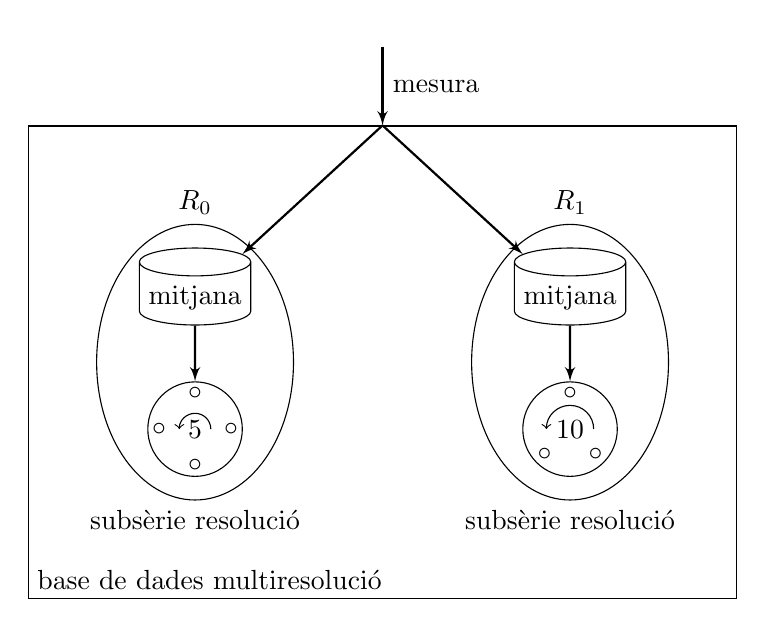
\begin{tikzpicture}
 \tikzset{
        myarrow/.style={->, >=latex',  thick},
      }
      

  \node[rectangle,draw,minimum height=6cm,minimum width=9cm] (m) {};
  \draw[shift=( m.south west)]   
  node[above right] {base de dades multiresolució};


  %discmig
  \node (m.center) (discr1) {};

  %discr
  
  \node[ellipse,draw,minimum height=3.5cm,minimum width=2.5cm,alias=discr0] [left=of discr1] {};
  \node[above=0cm of discr0.north] {$R_0$};
  \node[below=0cm of discr0] {subsèrie resolució};

  \node[cylinder, draw, shape border rotate=90, aspect=0.25,alias=buffer0] [below=3mm of discr0.north] {mitjana};
  \node[circle, draw,alias=disc0,minimum width=1.2cm]  [above=3mm of discr0.south] {5} ;
  \draw [->] (disc0.center)++(.2:.2cm) arc(0:180:.2cm);
  \draw[myarrow] (buffer0.bottom) -- (disc0.north);

  \node[circle,minimum width=9mm] (d0boles) [below=0mm of disc0.center,anchor=center] {};
  \node[below=0mm of d0boles.north,anchor=center] {$\circ$};
  \node[below=0mm of d0boles.east,anchor=center] {$\circ$};
  \node[below=0mm of d0boles.south,anchor=center] {$\circ$};
  \node[below=0mm of d0boles.west,anchor=center] {$\circ$};


  %discrd

  \node[ellipse,draw,minimum height=3.5cm,minimum width=2.5cm,alias=discrd] [right=of discr1] {};
  \node[above=0cm of discrd] {$R_1$};
  \node[below=0cm of discrd] {subsèrie resolució};

  \node[cylinder, draw, shape border rotate=90, aspect=0.25,alias=bufferd] [below=3mm of discrd.north] {mitjana};
  \node[circle, draw,alias=discd,minimum width=1.2cm]  [above=3mm of discrd.south] {10} ;
  \draw [->] (discd.center)++(.3:.3cm) arc(0:180:.3cm);
  \draw[myarrow] (bufferd.bottom) -- (discd.north);

  \node[circle,minimum width=9mm] (d1boles) [below=0mm of discd.center,anchor=center] {};
  \node[below=0mm of d1boles.north,anchor=center] {$\circ$};
  \node[below=0mm of d1boles.south east,anchor=center] {$\circ$};
  \node[below=0mm of d1boles.south west,anchor=center] {$\circ$};


  %mesura 
  \node[above=1cm of m.north] (m0) {};

  \draw[myarrow] (m0) -- (m.north) 
  node[right,midway] {mesura};

  \draw[myarrow] (m.north) -- (buffer0);
  \draw[myarrow] (m.north) -- (bufferd);


\end{tikzpicture}
\caption{Arquitectura de SGSTM particular per l'\autoref{ex:model:bdm1}}
\label{fig:model:ex1}
\end{figure}

L'arquitectura de la base de dades que conté aquesta sèrie temporal
multiresolució es pot veure a la \autoref{fig:model:ex1}. 
 L'esquema
de multiresolució que correspon als instants de consolidació, des de 0
fins a 30, és el següent:
\begin{itemize}
\item La subsèrie resolució $R_0$ serà consolidada en els instants 5,
  10, 15, 20, 25 i 30.
\item La subsèrie resolució $R_1$ serà consolidada en els instants 10,
  20 i 30.
\end{itemize}


Iniciem la base de dades a l'instant de temps 0, instant en el qual la
sèrie temporal multiresolució és $M_1^0 = \{ ( \{\} , \{\} , 0 , 5 ,4
, \text{mitjana} ) , ( \{\} , \{\} , 0 , 10 ,3 , \text{mitjana} ) \}$;
és a dir amb les sèries temporals buides i els darrers instants de
consolidació iniciats a 0.




A continuació, afegim a la sèrie temporal multiresolució les mesures
de la sèrie temporal $S_1=\{
(1,0),(5,0),(8,0),(10,0),(14,0),(19,0),(22,0),(26,0),(29,0) \}$. Tots
els valors valen zero per tal de centrar la comprensió de l'exemple en
l'estructura de temps de consolidació; pel que fa a exemples
d'agregació de valors es poden veure amb més detall a la
secció~\ref{sec:model:agregador}.


Si consolidem la sèrie temporal multiresolució cada cop que sigui
consolidable, és a dir en els instants que marca l'esquema de
multiresolució, a l'instant 29 després d'haver inserit la darrera
mesura la sèrie temporal multiresolució és $M_1^{29} = \{ (
\{(26,0),(29,0)\},\{(10,0),(15,0),(20,0),(25,0)\}, 25 , 5 ,4 ,
\text{mitjana} ), ( \{(22,0),(26,0),(29,0)\}, \{(10,0),(20,0)\},
20 , 10 ,3 , \text{mitjana} ) \}$.  Aquesta sèrie temporal
multiresolució es mostra a la \autoref{fig:model:stm} en forma de
taula.


Es pot observar que als buffers hi ha emmagatzemades les mesures
pendents de consolidar per a cada subsèrie i als discs les darreres
mesures consolidades:
\begin{itemize}
\item Per a la subsèrie resolució $R_0$ hi ha pendent de consolidar
  l'interval de temps $[25,30]$ i al disc hi ha emmagatzemades les 4
  mesures màximes permeses; és a dir que la que s'havia consolidat a
  l'instant $5$ ja s'ha perdut.
\item Per a la subsèrie resolució $R_1$ hi ha pendent de consolidar
  l'interval de temps $[20,30]$ i al disc hi ha emmagatzemades 2
  mesures. El disc encara no ha arribat al cardinal màxim $k=3$ degut
  a que la base de dades s'ha iniciat a l'instant $0$ i la primera
  consolidació d'aquesta subsèrie ha estat a l'instant $10$.
\end{itemize}




\begin{figure}[tp]
  \centering
  \begin{tabular}{|c|c|c|c|c|c|}
    \multicolumn{2}{c}{$M_1^{29}$} \\ \hline
    $S_B$  & $S_D$ & $\tau$ & $\delta$ & $k$ & $f$ \\ \hline
      \begin{tabular}{|c|c|}
         \hline
         $t$  & $v$ \\ \hline
         26  & 0 \\
         29 & 0 \\\hline
       \end{tabular} & 
      \begin{tabular}{|c|c|}
         \hline
         $t$  & $v$ \\ \hline
         10  & 0 \\
         15  & 0 \\
         20 & 0 \\ 
         25 & 0 \\\hline
       \end{tabular} 
       & 25 & 5  & 4 & mitjana  \\ \hline
       \begin{tabular}{|c|c|}
         \hline
         $t$  & $v$ \\ \hline
         22  & 0 \\
         26  & 0 \\
         29 & 0 \\\hline
       \end{tabular} & 
      \begin{tabular}{|c|c|}
         \hline
         $t$  & $v$ \\ \hline
         10  & 0 \\
         20  & 0 \\\hline
       \end{tabular}  
       & 20 & 10 & 3 & mitjana  \\ \hline
  \end{tabular}
  \caption{Taula d'una sèrie temporal multiresolució}
  \label{fig:model:stm}
\end{figure}

\end{example}


\begin{example} [Sèrie temporal multiresolució amb vistes]

  En el model relacional de SGBD molt sovint s'utilitzen vistes per a
  agrupar informació de vàries relacions, per a mostrar-ne una part,
  etc. Una vista és una variable relació virtual derivada d'una
  expressió relacional \parencite{date13}. En aquest exemple mostrem
  la mateixa sèrie temporal multiresolució de
  l'\autoref{ex:model:bdm1} però organitzada amb forma de vistes
  relacionals.


  Sigui $M_2^{\text{series}}= ((S':\text{nom},S:\text{sèrie
    temporal}),\{ (S_{B1},\{(26,0),(29,0)\}),
  (S_{B2},\{(22,0),(26,0),(29,0)\}),
  (S_{D1},\{(10,0),(15,0),(20,0),(25,0)\}),
  (S_{D2},\{(10,0),(20,0)\} )\})$ una relació de sèries
  temporals i noms, i $M_2'=
  ((S'_B:\text{nom},S'_D:\text{nom},\tau:\R,\delta:\R,k:\N,f:\text{funció}
  ),\{ (S_{B1},S_{D1},25 ,5 ,4 ,\text{mitjana} ), ( S_{B2},S_{D2},20 ,
  10 ,3 , \text{mitjana} ) \})$ una sèrie temporal multiresolució amb
  noms als atributs de sèries temporals; la vista de la sèrie temporal
  multiresolució es mostra a la \autoref{fig:model:stm:vistes} i es
  defineix com a
  \begin{align*}
    \text{vista } M_2 =& (M_2' \join ( M_2^{\text{series}} \rename S' \as S_B', S \as S_B )) \\
    &\join ( M_2^{\text{series}} \rename S' \as S_D', S \as S_D )
    \{\text{all but } S_B',S_D' \}
  \end{align*}




  \begin{figure}[tp]
    \centering
    \begin{tabular}{|c|c|c|c|c|c|}
      \multicolumn{2}{c}{$M'_2$} \\ \hline
      $S'_B$  & $S'_D$ & $\tau$ & $\delta$ & $k$ & $f$ \\ \hline
      $S_{B1}$ & $S_{D1}$ & 25 & 5  & 4 & mitjana  \\
      $S_{B2}$ & $S_{D2}$ & 20 & 10 & 3 & mitjana  \\ \hline
    \end{tabular}\qquad
    \begin{tabular}{|c|c|c|}
      \multicolumn{3}{c}{$M^{\text{series}}_{2}$} \\ \hline
      \multirow{2}{*}{$S'$}  &  \multicolumn{2}{c|}{$S$} \\ \cline{2-3}
      & $t$      & $v$  \\ \hline
      \multirow{2}{*}{$S_{B1}$} 
      & 26 & 0 \\ 
      & 29 & 0 \\ \hline
      \multirow{3}{*}{$S_{B2}$} 
      & 22 & 0 \\ 
      & 26 & 0 \\ 
      & 29 & 0 \\ \hline
      \multirow{4}{*}{$S_{D1}$} 
      & 10 & 0 \\ 
      & 15 & 0 \\ 
      & 20 & 0 \\ 
      & 25 & 0 \\ \hline
      \multirow{2}{*}{$S_{D2}$} 
      & 10 & 0 \\ 
      & 20 & 0 \\ \hline
    \end{tabular}
    \caption{Taula d'una sèrie temporal multiresolució amb vistes
      relacionals}
    \label{fig:model:stm:vistes}
  \end{figure}


  D'aquesta manera $M_2$ té els mateixos valors que la $M_1$ definida
  a l'exemple anterior; observant només el resultat de $M_2$ no es pot
  distingir que és una vista. Així doncs, les vistes ens permeten
  organitzar una sèrie temporal multiresolució de forma més còmoda i,
  a més tal com es descriu a \textcite{date13}, mantenint que totes
  les operacions i propietats que són d'aplicació a les relacions ho
  són també a les seves vistes.


%S'observa que per tal de complir amb les propietats de les relacions, totes les sèries temporals dels buffers han de ser del mateix tipus, és a dir tenir la mateixa capçalera. El mateix succeeix amb les sèries temporals dels discs. (Vegeu els exemples de la secció \ref{par:model:exemple-relvalues} sobre valors relació). No obstant les mesures que entren a la base de dades provenen de la mateixa sèrie temporal i per tant les sèries temporals emmagatzemades sempre seran del mateix tipus.



\end{example}



\begin{example} [Sèrie temporal multiresolució amb desfasaments]
\label{ex:model:bdm-desfasaments}

A l'\autoref{ex:model:bdm1} s'ha mostrat una sèrie temporal
multiresolució en la que la consolidació de les dues subsèries obeeix
a la mateixa funció d'agregador d'atributs $f$. En aquest exemple
treballem amb els mateixos valors que a l'\autoref{ex:model:bdm1} però
ara canviem la funció de la segona subsèrie resolució per un agregador
amb desfasament; és a dir que cada cop que consolida retorna una
mesura amb un retard d'una certa durada. Aquest nou agregador que
anomenem \emph{mitjanad5} també fa la mitjana però amb un desfasament
de $5$ unitat de temps, a l'apartat
\ref{sec:model:sgstm-manipulacio-esquema} es defineix amb més precisió
aquest concepte de desfasament.


Seguint el mateix procediment que a l'\autoref{ex:model:bdm1}, a
l'instant 29 després d'haver inserit la darrera mesura la sèrie
temporal multiresolució és $M_3^{29} = \{ ( \{(26,0),(29,0)\} ,
\{(10,0),(15,0),(20,0),(25,0)\} , 25 , 5 ,4 , \text{mitjana} ) , (
\{(19,0),(22,0),(26,0),(29,0)\} , \{(5,0),(15,0)\} , 20 , 10 ,3 ,
\text{mitjanad5} ) \}$.  Aquesta sèrie temporal multiresolució es
mostra a la \autoref{fig:model:stm:desfasaments} en forma de taula.


\begin{figure}[tp]
  \centering
  \begin{tabular}{|c|c|c|c|c|c|}
    \multicolumn{2}{c}{$M_3^{29}$} \\ \hline
    $S_B$  & $S_D$ & $\tau$ & $\delta$ & $k$ & $f$ \\ \hline
      \begin{tabular}{|c|c|}
         \hline
         $t$  & $v$ \\ \hline
         26  & 0 \\
         29 & 0 \\\hline
       \end{tabular} & 
      \begin{tabular}{|c|c|}
         \hline
         $t$  & $v$ \\ \hline
         10  & 0 \\
         15  & 0 \\
         20 & 0 \\ 
         25 & 0 \\\hline
       \end{tabular} 
       & 25 & 5  & 4 & mitjana  \\ \hline
       \begin{tabular}{|c|c|}
         \hline
         $t$  & $v$ \\ \hline
         19  & 0 \\
         22  & 0 \\
         26  & 0 \\
         29 & 0 \\\hline
       \end{tabular} & 
      \begin{tabular}{|c|c|}
         \hline
         $t$  & $v$ \\ \hline
          5  & 0 \\
         15  & 0 \\\hline
       \end{tabular}  
       & 20 & 10 & 3 & mitjanad5  \\ \hline
  \end{tabular}
  \caption{Taula d'una sèrie temporal multiresolució amb desfasaments}
  \label{fig:model:stm:desfasaments}
\end{figure}



Així doncs, mentre que l'esquema de multiresolució segueix sent el
mateix pel que fa als instants de consolidació, els instants de temps
de la sèrie temporal emmagatzemada a la subsèrie resolució $R_1$ tenen
un retard de $5$ unitats de temps.  Per una banda, es pot observar a
la $S_{B2}$ que el buffer ara és 5 unitats més gran i emmagatzema
mesures de l'interval $[15,30]$. Per altra banda, es pot observar a la
$S_{D2}$ que els instants emmagatzemats són $5$ i $15$ corresponents
als instants de consolidació $10$ i $20$. Pel que fa a la resta de
valors, no han variat respecte de l'\autoref{ex:model:bdm1}.



\end{example}


%%% Local Variables: 
%%% mode: latex
%%% TeX-master: "main"
%%% End: 

% LocalWords:  buffers multiresolució agregador l'agregador subsèries
% LocalWords:  d'agregador



\section{Implementacions}
\begin{frame}{Experimentació: implementacions}

  \begin{itemize}
  \item Implementació de referència, orientada a objectes mitjançant Python
  \item Implementació para\l.lela i distribuïda amb MapReduce mitjançant Hadoop
  \item Implementació relacional amb Tutorial D mitjançant Rel
  \end{itemize}



Comparació qualitativa:

  \begin{itemize}
  \item Totes obtenen els mateixos resultats
  \item Implementació reduïda per tal d'ajustar-se a MapReduce
  \item Implementació Tutorial D és acadèmica, no per a producció
  \item Implementació para\l.lela no permet computació incremental
  \item Implementacions amb pèrdua requereixen planificar l'esquema de multiresolució
  \end{itemize}


\end{frame}


%%% Local Variables: 
%%% mode: latex
%%% TeX-master: "defensa"
%%% End: 


\section{Casos d'ús}

\begin{frame}{Casos d'ús}

  \begin{enumerate}
  \item Funció de multiresolució
  \item Sistemes duals
  \item Avaluació de la qualitat de la multiresolució
  \end{enumerate}

\end{frame}


\subsection*{Variacions}

\begin{frame}{SGSTM vs.\ funció de multiresolució}


Model sistema de gestió de bases de dades (conserva estat):


\begin{center}
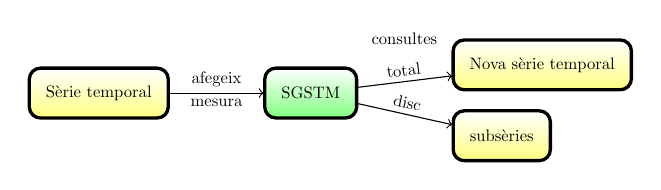
\begin{tikzpicture}[scale=0.6, every node/.style={transform shape}]

      \tikzset{
        mynode/.style={rectangle,rounded corners,draw=black, 
          very thick, inner sep=1em, minimum size=3em, text centered,
          groc},
        myarrow/.style={->, shorten >=1pt, thick},
        mylabel/.style={text width=7em, text centered},
        groc/.style={top color=white, bottom color=yellow!50},
        verd/.style={top color=white, bottom color=green!50},
        roig/.style={top color=white, bottom color=red!50},
      }  






 \node[mynode] (S) {Sèrie temporal};
 \node[mynode, verd, right=2cm of S] (sgstm) {SGSTM};
 \node[mynode, above right=-0.5cm and 2cm of sgstm] (Sp) {Nova sèrie temporal};
 \node[mynode, below=1.5cm of Sp.west, anchor=west] (S1) {subsèries};

 \draw[->] (S) -- (sgstm) node[above,midway,sloped] {afegeix} node[below,midway,sloped] {mesura}; 
 \draw[->] (sgstm) -- (Sp) node[above,midway,sloped] {total}; 
 \draw[->] (sgstm) -- (S1) node[above,midway,sloped] {disc}; 
 \node[left=2.1cm of Sp.north] (consultes) {consultes};

\end{tikzpicture}
\end{center}




Model d'operació de multiresolució (sobre un SGST):


\begin{center}
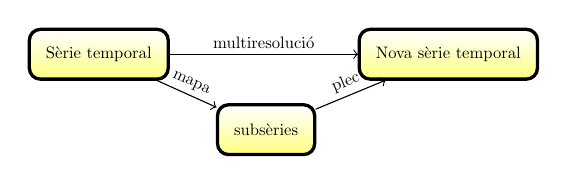
\begin{tikzpicture}[scale=0.6, every node/.style={transform shape}]

      \tikzset{
        mynode/.style={rectangle,rounded corners,draw=black, 
          very thick, inner sep=1em, minimum size=3em, text centered,
          groc},
        myarrow/.style={->, shorten >=1pt, thick},
        mylabel/.style={text width=7em, text centered},
        groc/.style={top color=white, bottom color=yellow!50},
        verd/.style={top color=white, bottom color=green!50},
        roig/.style={top color=white, bottom color=red!50},
      }  






 \node[mynode] (S) {Sèrie temporal};
 \node[mynode, right=4cm of S] (Sp) {Nova sèrie temporal};
 \draw[->] (S) -- (Sp) node[above,midway] {multiresolució}; 

 \node[mynode, below right=0.5cm and 1cm of S] (S1) {subsèries};
 \draw[->] (S) -- (S1) node[above,midway,sloped] {mapa}; 
 \draw[->] (S1) -- (Sp) node[above,midway,sloped] {plec}; 


\end{tikzpicture}
\end{center}


\end{frame}




% \begin{frame}{Usos de la multiresolució}

% Possibilitats de computació:

%   \begin{itemize}
%   \item Computació offline
%   \item Computació incremental
%   \item Computació para\l.lela (offline)
%   \item Computació distribuïda (xarxes de sensors)
%   \end{itemize}


% Arquitectures dels sistemes:
%   \begin{itemize}

%   \item Únicament SGSTM: emmagatzematge amb pèrdua, aproximació a l'històric, dades originals no són necessàries.
%   \item SGST+SGSTM: dipòsit a llarg termini poc consultat i sistema per a resoldre consultes habituals o visualitzacions immediates
%   \item Funció de multiresolució (para\l.lela): experimentació 
%   \end{itemize}


% \end{frame}



\begin{frame}{Sistemes duals}




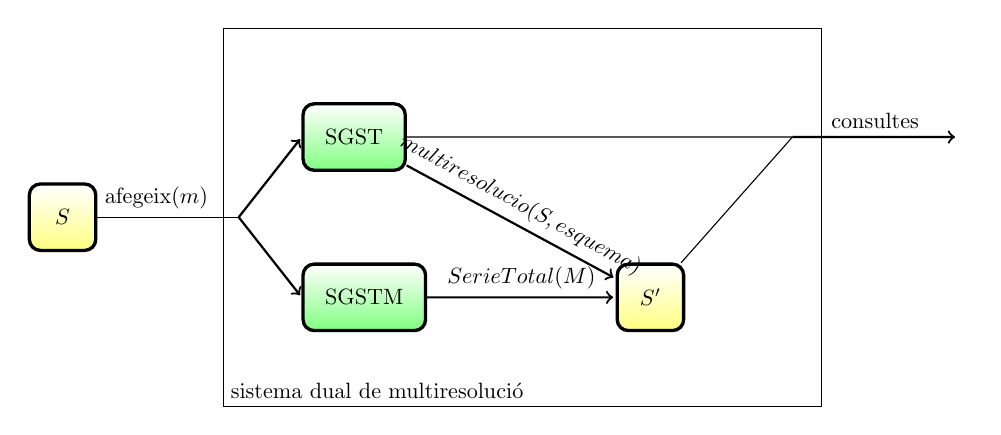
\begin{tikzpicture}[scale=0.8, every node/.style={transform shape}]

      \tikzset{
        mynode/.style={rectangle,rounded corners,draw=black, 
          very thick, inner sep=1em, minimum size=3em, text centered,
          groc},
        myarrow/.style={->, shorten >=1pt, thick},
        mylabel/.style={text width=7em, text centered},
        groc/.style={top color=white, bottom color=yellow!50},
        verd/.style={top color=white, bottom color=green!50},
        roig/.style={top color=white, bottom color=red!50},
      }  






 \node[mynode] (m) {$S$};

 \node[right=2cm of m] (mdins) {};

 \node[mynode, verd, above right=0.6cm and 1cm of mdins] (tsms) {SGST};

 \node[mynode, verd, below right=0.6cm and 1cm of mdins] (mtsms) {SGSTM};

 \node[rectangle,draw,minimum height=6cm,minimum width=9.5cm,right=-0.25cm of mdins] (dual) {};

\draw[shift=( dual.south west)]   
  node[above right] {sistema dual de multiresolució};






 \node[mynode,right=3cm of mtsms] (ts) {$S'$};



 \draw (m.east) -- (mdins.east) node[above right,at start]
 {afegeix$(m)$};

 \draw[myarrow] (mdins.east) -- (tsms.west);
 \draw[myarrow] (mdins.east) -- (mtsms.west);


 \draw[myarrow] (tsms) -- (ts) node[above,midway,sloped]
 {$multiresolucio(S,\text{esquema})$}; 
 
 \draw[myarrow] (mtsms) -- (ts) node[above,midway,sloped]
 {$SerieTotal(M)$};




 \node[right=6cm of tsms] (consdins) {};

 \draw (tsms) -- (consdins.center);
 \draw (ts) -- (consdins.center);

 \node[right=2.5cm of consdins] (consultes) {};
 \draw[myarrow] (consdins.center) -- (consultes) node[above,midway,sloped]
 {consultes};



\end{tikzpicture}

Conceptes relacionats: 
\begin{itemize}
\item Arquitectura Lambda \parencite{marz14:bigdata} 
\item Precomputació de vistes \parencite{date04:introduction8}
\end{itemize}





\end{frame}




\subsection*{Teoria de la informació}
\begin{frame}{Avançaments en determinar la qualitat de la multiresolució}

  Quantificació de l'error que es comet en la selecció de la informació
  per a la muliresolució. 

\begin{block}{Definició del problema}
\centering
consulta(sèrie temporal original) vs.\ consulta(multiresolució)
\end{block}


Alguns dels escenaris particulars analitzats:
\begin{itemize}
\item Consulta a tota la sèrie temporal i mateixa consulta i atribut:
  \begin{itemize}
  \item Màxim i total no tenen error
  \item Mitjana té error
  \item Mitjana en el cas d'una sèrie temporal regular no té error 
  \end{itemize}

\item Consultes d'un interval determinat:
  \begin{itemize}
  \item Interval múltiple de les resolucions consolidades: similar al punt anterior
  \item No múltiple: hi ha error. Fitat per a variables monòtones creixents.
  \end{itemize}

% \item Conservació dels totals en comptadors

% \item Equivalència de l'atribut mitjana en sèries temporals regulars per a diversos mètodes de representació.

\end{itemize}

\end{frame}




%%% Local Variables: 
%%% mode: latex
%%% TeX-master: "defensa"
%%% End: 
%  LocalWords:  multiresolució



\section{Conclusions}
\begin{frame}{Conclusions}

  \begin{itemize}
  \item S'ha situat l'estat actual de l'emmagatzematge i del tractament de sèries temporals.

  \item S'ha estudiat el sistema de gestió de bases de dades RRDtool.

  \item S'ha dissenyat un model que descriu l'estructura i el
    comportament dels SGBD Round Robin per a sèries temporals.
  
  \item S'ha proposat una implementació de referència del model dissenyat.


 \item Un SGBD Round Robin és un sistema informàtic d'emmagatzematge d'una sèrie temporal compactada i repartida segons diferents funcions d'interpolació i períodes de mostreig.

  \end{itemize}

\end{frame}




\begin{frame}{Treball futur}

\begin{itemize}

\item A partir del model RRD es poden estudiar l'aplicació de tècniques d'anàlisis de sèries temporals  i es poden dissenyar SGBD RRD assegurant el funcionament desitjat.


\item Tractament de dades desconegudes. Interpoladors específics.

\item Operacions de consulta: extreure dades, fusionar sèries temporals, visualització, predicció, cerca de patrons, etc.

\item Configurant els interpoladors i els períodes de mostreig s'aconsegueixen reduccions diferents de les sèries temporals.

\item Comprovació amb dades experimentals, (\cite{keogh02}).

\item Variacions en la implementació del model per complir restriccions.

\end{itemize}
\end{frame}


\begin{frame}

\begin{center}
{\huge
Gràcies per l'atenció!
}
\end{center}

\end{frame}

%%% Local Variables: 
%%% mode: latex
%%% TeX-master: "presentacio"
%%% End: 



\begin{frame}<handout:0>
  \addtocounter{framenumber}{-1}

  \begin{center}
    {\huge
      Gràcies per l'atenció!
    }
  \end{center}

\end{frame}


\appendix


\begin{frame}[allowframebreaks]{Referències}

\printbibliography

\end{frame}


\end{document}


%%%%%%%%%%%%%%%%%%%%%%%%%%%%%%%%%%%%%%%%%%%%%%%%%%%%%%%%%%%%%%%%%%%%%%%%%%  
% Defensa Tesi Doctoral. 
%
% Copyright (C) 2011-2015 Aleix Llusà Serra.
% 
% This LaTeX document is free software: you can redistribute it and/or
% modify it under the terms of the GNU General Public License as
% published by the Free Software Foundation, either version 3 of the
% License, or (at your option) any later version.
%
% This document is distributed in the hope that it will be useful, but
% WITHOUT ANY WARRANTY; without even the implied warranty of
% MERCHANTABILITY or FITNESS FOR A PARTICULAR PURPOSE. See the GNU
% General Public License for more details.
%
% You should have received a copy of the GNU General Public License
% along with this document. If not, see <http://www.gnu.org/licenses/>.
%
%
% Aleix Llusà Serra
% Departament de Disseny i Programació de Sistemes Electrònics de la Universitat Politècnica de Catalunya (DiPSE-UPC)
% Escola Politècnica Superior d'Enginyeria de Manresa (EPSEM)
% Av. de les Bases de Manresa, 61-73
% 08242 Manresa (Barcelona)
% PAÏSOS CATALANS 
%
% aleix (a) dipse.upc.edu
% 
% El codi font LaTeX del document es troba a 
% <http://escriny.epsem.upc.edu/projects/rrb/>
%%%%%%%%%%%%%%%%%%%%%%%%%%%%%%%%%%%%%%%%%%%%%%%%%%%%%%%%%%%%%%%%%%%%%%%%%% 